\chapter{Аланы}

С годами меняется облик планеты. Народы расселяются, обретают другие имена, обычаи, веру и даже языки, сохраняя нечто старое и предлагая соседним народам свои слова, обычаи и веры взамен приобретенных.

В Чечне, в зеленом подгорьи, у берега реки Сунжи есть село Алхан-кала. В глубокое прошлое проросли его корни. А в 19 веке Чеченцы переселись отсюда к юго-востоку, по другую сторону реки, и основали Алхан-Юрт, а на месте прежней Алхан-калы возникла станица терских казаков Ермоловская. Некоторое время атаманил в ней дед моей бабушки по отцовской линии, Леонтий Никитин. В начале 1920-х станица забунтила вместе с прочими окрестными. И по приказу Орджоникидзе ее жителей кого выселили, кого услали. Прошли годы. Ныне это снова Алхан-кала, и обитают в ней Чеченцы.

В четырех километрах от Алхан-калы найдено крупнейшее в том краю городище – остатки города, в котором жили, как полагают, Аланы – народ, ответвившийся от Сарматов. Укрепление длиной в километр, обнесенное рвами, один из коих глубиной 9 метров. Мощеная булыжниками мостовая. Кто ходил по ней? Чья речь слышалась? А в окрестных селениях?

Тот же вопрос уместно задать о Киевщине.

Как принято считать, Киев основан братьями Кием, Хоривом, Щеком да сестрой их Лыбедью. Одни ученые принимают это летописное предание, другие опровергают. Нет общего мнения.

Вот знаменитый историк Василий Ключевский. Его живо изложенные лекции в печатном виде зачитывались до дыр. Ключевский оценивал основание Киева скромно, приурочивая его к Кию с братьями, невесть почему назвав их звероловами и поселив в некие однодворные деревни: 

\begin{quotation}
Так Киев возник из трех однодворных деревень с общим укрепленным убежищем, которые поставлены были тремя звероловами...
\end{quotation}

Историки, согласные в определенной мере с преданием о братьях, обычно далее того не идут. Заложили братья крепость – град Киев, и ладно. А прежде что тут было? Ученые уходят от прямого ответа. Отделываются размытыми словами. Да, первобытные стоянки времен палеолита. Да, защитные валы черняховской культуры. Черепки горшков трипольской культуры... Но город, дескать, возник только при Кие.

Пытливый Максим Берлинский в своем «Кратком описании Киева»\cite{berl01} предположил наличие тут города до основания крепости Киева, ссылаясь на Клавдия Птолемея, перечислявшего города, лежащие по Борисфену, как Греки называли Днепр\footnote{Наука использует два основных способа чтения букв древнегреческих текстов, «итацизм» да «этацизм». По первому, слово Βορυσθένης надо читать как Ворисфенес, по второму – Борисфенес. Однако никто точно не знает, каково было произношение у древних Греков. Кроме того, в переводах прижилось отбрасывание окончания «ес», остается лишь корень Борисфен. Можно считать, что любое название либо имя из давних сочинений Греков переведено приблизительно. Оно могло произноситься иначе! Кстати, согласно поэме римского императора Адриана, имя коня Цезаря было Борисфен Аланский.}:

\begin{quotation}
Птолемей, между прочими городами упоминает об Амадоке, стоявшем при повороте Днепра, по левую его сторону, близ какого-то озера, или вероятнее реки, что по его ландкарте придется при впадении Десны в Днепр. И по ту же сторону Днепра, выше сего, упоминает о находившемся городе Азагориум, может быть, от тогдашних тамошних жителей назывался Загорье.
\end{quotation}

А один из самых передовых людей времен Петра I, многообразный деятель Василий Татищев, трактуя некий вариант карты к «Географии» Птолемея, название Азагориум примерял к Переславлю, а вот Амадок – относил к Киеву.

Попробуем разобраться с этим сами, по трудам давних греческих историков и географов, а также правителей Византии. Все их труды относятся ко времени, когда в наших краях жили Скифы (они же Скиты) и Сарматы. Выяснение подробностей приведет нас к другим источникам, мы возьмем на вооружение свидетельства давних Арабов, Латинов, Французов, а также наших летописцев и толмачей.

Задача – не раскрыть тайны прошлого до конца, но пробовать найти подступы к этому прошлому. Сравним то, что говорит современная наука, с тем, что утверждают люди, общавшиеся со Скифами и другими народами древности непосредственно.

Спросите любого на улице, кто такие Скифы? Вообще-то прохожего это вообще не колышет. Но упрощенное представление таково – древний воинственный народ. Кочевали по степям, хоронили своих в курганах, были мастерами делать украшения из золота, снимали с врагов скальпы.

А что скажет наука? Она завороженно твердит, что Скифы – «ираноязычные племена», обитавшие в землях от Дона до Дуная с 8 века до нашей эры по 9 век нашей эры.

Отметим, что теперь на большей части этого пространства живут сплошь Славяне – Чехи, Поляки, Русские, Украинцы – словом все нынешние страны со славянским населением прежде составляли Скифию.

Летописец Нестор в Повести временных лет, перечислив славянские народы, что обитают в землях от Дунаю до Днепра, пишет, что до сего дня Греки называют эти места «Великая Скуфь» (Большая Скифия). И повторно он говорит, о составе похода Вещего Олега, что Олег набрал войско из народов Варяг, Словен, Чуди, Кривичей, Мери, Полян, Северов, Древлян, Радимичей, Хорватов, Дулебов, Тиверцов – «си вси звахуться Великая Скуфь» – поясняет Нестор.

Так выходит, Скифы – общее греческое название Славян? А как же «ираноязычные племена»? В пользу ираноязычия Скифов говорят, казалось бы, имена рек – Дунай, Дон, Днепр, Днестр, многочисленные Донцы (Северский, Липовый, Саженный) – где ученые усматривают скифское слово «дан», что переводят как «вода» либо «река». А «Днепр», он же «Данапр» – мол, это «дана» и «апр», два скифских слова, означающих вместе вода глубокая.

А предложу-ка две славянские трактовки речных имен. Мы имеем весьма мокрый корень «дно». Отсюда, кстати, и «тонуть» – «донуть», идти ко дну. Разница между звуками «т» и «д» невелика. При склонении, «дон» легко превращается в «дне». Далее, вот корень иного, временного рода – «день», «дни». Быть может, название большой реки составлялось из производного от слова «дней» и указания количества дней пути по этой реке, то есть известной длины реки. Все эти «пр», «стр» – не искаженные ли числа?

Что мы знаем о языке, на котором говорили Скифы? Всеволод Миллер и Василий Абаев в своих работах, справедливо полагая современных Осетинов потомками Скифов (через Сарматов и Аланов, Асов), скифский язык пытались восстановить посредством осетинских наречий – иронского и дигорского. 

А как же Великая Скуфь? В ее пределах скифский язык улетучился, не оставив иного следа, кроме названий рек?

%Но что дошло до наших дней от языка Скифов? Их имена в сочинениях на греческом
%Будто бы – названия рек. Что еще? Ничего.

%Две крайности. По одной Скифы – греческое название Славян. По другой – ираноязычные кочевники.

%Названия рек хорошее подтверждение тому, что Скифы пользовались словами с иранской основой для обозначения рек, лежащих на огромном расстоянии друг от друга. Причем имена эти сохраняются поныне, значит, были местными! Не называем же мы Днепр как древние Греки – Борисфеном. В русском и украинском языках примесь, трактуемая «иранской», касается не только воды, это еще и некоторые цвета.

Общепринятое знание сбивает с толку. Это ведь ученые, а не сами Скифы, сказали нам про иранские корни в названиях рек. Может они вовсе не иранские, а утраченные славянские, либо следы какого-то третьего языка. Как вообще языки влияют друг на друга? А подобно музыкальным жанрам, при этом степень возможного влияния зависит от совместимости жанров.

Наука полагает, что Скифов вытеснили Сарматы, тоже ираноязычные. И разделяет Скифов, Сарматов, да Славян – причем то временами, то происхождением. 

Но я больше доверяю давним Грекам. Они, в отличие от современных ученых, общались со Скифами. Есть что рассказать. Поэтому обратимся за сведениями к Геродоту, Страбону, Льву Диакону, Клавдию Птолемею и Плинию Старшему.

Хотел расставить эти источники по времени, однако из-за путаницы с летосчислением я не могу доверять общепринятым датировкам сих трудов, и способен упорядочить оные лишь относительно. Например, Страбон упоминает Геродота – значит, «История» Геродота написана раньше, чем «География» Страбона. Географические сведения Греков существенно отличаются не только от нынешних, но и друг от друга, что впрочем может отражать изменения, происходящие с местностью с течением времени, а не ошибочность представлений.

К рукописным сочинениям Греков нередко прилагались карты, однако неясно, составлены ли они по карте самого сочинителя, либо на основании его текста. Подлинники, начертанные Клавдием Птолемеем и другими остаются неизвестными, да и вряд ли сохранились бы. Пожары, сырость, прочие влияния окружающей среды, наконец невольный враг древних знаний – мыши.

Старинные карты кажутся на первый взгляд нелепыми. Причина тому, кроме ошибок, смешение источников современных составителю карты и источников буквально допотопных, отражающих состояние Земли до Потопа, который, сопровождаемый другими бедствиями, вполне мог служить причиной исчезновения одних гор и морей, возникновения других, переменить течения рек, не говоря уже о том, что с лица земли стёрлись целые страны. Но водная сеть меняется быстро и без привлечения Потопа.

Таким образом наиболее древние карты давали одновременно представление о Земле до Потопа и после, а с течением времени уточняясь новыми данными, лишались допотопных следов. Поэтому чем ближе к нам, тем менее фантастичны карты.

В историко-географических трудах Греки по-своему обозначали страны, города, реки, моря и озера. Порой эти названия были искаженными производными от местных именований. Либо чисто греческими. А может, по-гречески их тогда называли и тамошние обитатели. И сейчас исследователи ломают себе головы, что же подразумевали греки?

Например, Рипейские (Рифейские) горы. С ними ученые соотносят Урал, Кавказ и Тянь-шань. Каравай, каравай, кого хочешь – выбирай. Но и некоторые Греки, тот же Страбон, вообще сомневались в существовании таких гор!

В «Географии» Птолемея, где употреблена сеть координат, устье Борисфена (Днепра) лежит западнее реки Хипаниса (в отечественных переводах часто пишут: «Гипанис»). С Хипанисом отождествляют Южный Буг, однако у Птолемея это разные реки, он различает Хипанис и «Буц» (Buces). Современные толкователи обычно пишут – Птолемей ошибается, устье Буга западнее устья Днепра.

Но если считать устьем Днепра западную часть современного Днепровского лимана (куда впадает и Днепр, и Южный Буг), то устье Днепра таки западнее, чем устье Буга. А Греки так и считали.

Археологи уже давно и обстоятельно раскапывают  древний город Ольвию\footnote{46°41'33.0"N 31°54'13.0"E}. Она лежит под Николаевом, на берегу Южного Буга, примерно в 5 километрах выше его устья в Днепровском лимане. Это именно Ольвия, о чем свидетельствуют найденные там многочисленные надписи на греческом. Вырезанные в камне, они подтверждают различные права вроде этого\cite{olbia01}:

\begin{quotation} 
В добрый час! Ольвиополиты дали Ксантиппу, сыну Аристофонта, эрхиейцу, сыну Филополида, дейрадиоту – афинянам, им самим и потомкам их проксению, право гражданства, освобождение от пошлин на все товары, какие бы ни ввезли или не вывезли они сами, или их дети, или братья, у которых отцовское имущество общее, или слуги, и дали право входа в гавань и выхода из гавани и в мирное, и в военное время, без конфискации и без заключения договора.
\end{quotation} 

Здесь мы видим слова без перевода (дейрадиот, проксений) – их точное значение остается неясным поныне, посему оставляют как есть. А вот «ольвиополиты» значит «жители Ольвии». Эти ольвиополиты часто упомянуты в надписях Ольвии, и можно сделать однозначный вывод о названии города.

%Плиний в 26-й главе «Естественной истории» говорит:
Плиний в «Естественной истории» говорит:

\begin{quotation}
На расстоянии 120 миль от Тира лежит река Борисфен, с одноименным озером и народом, а также городом на материке, на расстоянии 15 миль от моря. Старые названия этого города Олвиополис и Милетополис.
\end{quotation}

Тир это Днестр. Есть на нем город Тирасполь, что подтверждает отождествление Днестра с Тиром.

Итак, по Плинию, в 15 милях от устья Днепра  лежит город Борисфен, другие названия коего – Ольвия и Милетополь. Местных жителей именовали Борисфенитами. При пересчете в километры, 15 миль Плиния – это примерно расстояние от устья Днепровского лимана до Ольвии. Стало быть, сей лиман Греки принимали за часть Днепра.

Страбон, в 7-й книге «Географии» сообщает:

\begin{quotation}
Дельта Борисфена (Βορυσθένης) судоходна на 600 стадий, а близко другая река, Хипанис (Ὕπανις), и остров перед устьем Борисфена, с портом. Если плыть по Борисфену 200 стадий будет одноименный с рекой город: он называется также Олвиа, большой торг, основанный Милисиами.
\end{quotation}

%Εἶτα Βορυσθένης ποταμὸς πλωτὸς ἐφ᾽ ἑξακοσίους σταδίους καὶ πλησίον ἄλλος ποταμὸς Ὕπανις καὶ νῆσος πρὸ τοῦ στόματος τοῦ Βορυσθένους, ἔχουσα λιμένα. Πλεύσαντι δὲ τὸν Βορυσθένη σταδίους διακοσίους ὁμώνυμος τῶι ποταμῶι πόλις· ἡ δ᾽ αὐτὴ καὶ Ὀλβία καλεῖται, μέγα ἐμπόριον, κτίσμα Μιλησίων.

Как видим, и здесь Ольвия помещена на берегу именно Днепра. Даже указано расстояние к ней – 200 стадий. А устье Борисфена судоходно (вероятно для морских, не речных кораблей) на 600 стадий. Сколько всё это в пересчете?

По представлениям науки, 1 стадия это... Различают разные стадии. Греческая, мол, 178 метров, олимпийская 192,3 метра, аттическая – 177,6, птолемеева – 185 метров, и прочие. Беда! 

Возьмем округленное 180 метров. Сколько будет в километрах – 200 стадий? 200*180/1000 = 36 километров. Это расстояние от устья Днепровского лимана до Ольвии. Итак, Греки однозначно полагали, что устье Днепра – это устье нашего Днепровского лимана. А вот Ольвия лежала на берегу этого «продленного» Днепра. Где тогда находилось устье Южного Буга, я не знаю.

Вычислим теперь, на какое расстояние от моря судоходна дельта Днепра во время Страбона. 600 стадий умножим на 180 метров – равно 108000 метров. 108 километров. Принимая за устье Днепра устье нынешнего Днепровского лимана, и что русло проходило так же, как ныне, у нас получится, что суда от моря могли подниматься по дельте Днепра  немногим, километров на 20, выше Херсона.

%Геродот, живший раньше Страбона, утверждает, что Днепр известен на 40 дней пути. Но к этому мы еще вернемся.

Однако, Днепр был известен и выше – Геродот говорит, что на сорок дней пути! Геродот из наших греческих источников древнейший. Считается, что он жил в пятом веке до нашей эры, но я полагаю, что не столь давно. В своей «Истории», в книге «Мельпомена» он рассказывает о походе царя Персов Дария на Скифов, и дает обстоятельное описание последних\cite{herodotus01}:

\begin{quotation}
По словам самих Скифов, они – юнейший из всех народов, и о своем происхождении рассказывают так: первым человеком в этой стране, тогда еще пустынной, был Таргитай\footnote{Такое же имя, искаженное в «Таргитий», встречаем у Фиофилакта Симокатты в «Истории», где Таргитий – посол Аваров, пришедший к Ромеям-византийцам за ежегодной данью для кагана Аваров. Прочие имена Аваров по этому сочинению: Сирмий, Баян, Турум, Спарзевгун, Кунаксолан, Тулдих. Впрочем, Симокатта считает европейских Аваров самозванцами, на деле представителями народов Уар и Хунны.}; родителями Таргитая они называют, чему я не верю, Зевса и дочь реки Борисфенеса. Такое происхождение приписывается Таргитаю.

У него было три сына: Липоксаис, Арпоксаис и самый младший Колаксаис. При жизни их упали с неба на скифскую землю золотые предметы: плуг, ярмо, секира и чаша.

Первым увидел эти предметы самый старший из братьев; он приблизился к ним с целью взять, но при его приближении золото воспламенилось, и он отступил назад. Затем подошел средний брат, но с золотом повторилось то же самое. Таким образом золото горением не своим не допустило к себе двух братьев; с приближением третьего, наимладшего брата золото потухло, и он отнес его к себе в дом. Поэтому старшие братья согласились уступить наимладшему все царство.

От Липоксаиса, рассказывают дальше, произошли те из Скифов, которые носят название рода Авхатов (Αὐχάται), от среднего, Арпоксаиса, произошли Скифы, именуемые Катиарами или Трапиями (Κατίαροί τε καὶ Τράσπιες), а от наимладшего, царя, те, что называются Паралатами (Παραλάται). 

Общее название всех Скифов, по имени царя их, Сколоты (Σκολότους); Скифами назвали их Эллины\footnote{Я бы перевел иначе: общее название этих варваров – Сколоты, то есть из царского рода (царствующие), а Скифами их назвали Эллины. σύμπασι δὲ εἶναι οὔνομα Σκολότους, τοῦ βασιλέος ἐπωνυμίην. Σκύθας δὲ Ἕλληνες ὠνόμασαν.}.

Так рассказывают Скифы о своем происхождении, полагая, что от начала их существования или от первого царя Таргитая до похода Дария прошло круглым счетом никак не больше тысячи лет.

Упомянутое выше священное золото цари оберегают  весьма ревниво и ежегодно благоговейно чтут его обильными жертвоприношениями.
\end{quotation}

Здесь Геродот называет Царскими (по-скифски Сколотами), не всех Скифов вообще, а три скифских народа, ветви Скифов: Катиары, Трапии и Паралаты. Были и другие народы Скифов, над которыми, надо полагать, при Дарии властвовали эти Царские Скифы.

Вероятно, именование Царских Скифов перемещалось позже со Сколотов на другой народ из числа Скифов. Был один правящий народ, собиравший дань, и его подчиненные. Приск Панийский из Фракии, состоявший в посольстве Максимина к Аттиле, в «Истории Готфов»\footnote{Приск попутно дает имена Царских скифов, помимо Аттилы: Васих, Курсих, Верих. Жену Аттилы зовут Крека. Если в мужских именах поменять «х» на «ч», получим ближе к славянским: Васич, Курсич, Верич.} относит к Скифам народы Унны (Хунны) и Готфы (Готы), однако различает эти два народа, а Уннов величает Царскими Скифами. Как я понимаю из описания Приском сборного скифского войска, Унны и Готфы были родственны, но Готфы находились в подчинении у более хищных Уннов. Не исключаю, что те, кто при Геродоте именовались Сколотами, во время Аттилы слыли Хуннами.

Скифские народы, по Геродоту, живут от Истра (Дуная) до Танаиса (Дона)\footnote{С Танаисом связана странность. Историк Иордан в «Гетике» говорит, что есть два Танаиса. Один, разделяющий Европу с Азией, начинается в Рифейских горах и впадает в Мэотийское болото (оно отождествляется с Азовским морем). Этот Танаис никогда не замерзает, в отличие от соседних рек, а также Мэотиды и Босфора. А другой Танаис рождается в Хриннских горах и впадает в Каспийское море.}. Он называет следующие реки Скифии, кажется по порядку соединения их устий с морем, с запада на восток: Истрон (Ἴστρον), Тирас (Τύρης), Хипанис (Ὕπανις), Борисфенес (Βορυσθένης), Пантикапес (Παντικάπης), Хипакирис (Ὑπάκυρις), Геррос (Γέρρος, рукав Борисфена, впадает в Ипакирис), Танаис (Τάναϊς)\footnote{Всё это греческие и «огреченные» названия, поэтому даю как в подлиннике. Однако видно, что например Дон, Дан превращен в Танаис заменой «д» на «т» и добавлением «аис». «Тирас» же – греческое именование Днестра, ничего не переиначено.}. Про Хипанис сказано ранее, а отождествление Пантикапеса, Хипакириса и Герроса с современными названиями остается загадкой поныне.

Про Скифов Геродот пишет:

\begin{quotation}
Ведь у Скифов нет ни городов, ни укреплений, и свои жилища они возят с собой. Все они конные лучники и промышляют не земледелием, а скотоводством; их жилища – кибитки.
\end{quotation}

Казалось бы, здесь говорится вообще обо всех Скифах как о кочевниках. Однако почитаем «Историю» дальше. Я буду делать выдержки и свои отступления, чтобы обсудить. Среди скифских рек Геродот особенно хвалит Днепр:

\begin{quotation}
Четвертая река Борисфенес – из скифских рек после Истра наибольшая и, по нашему мнению, самая богатая полезными предметами не только между скифскими реками, но между всеми вообще, кроме впрочем египетского Нила; с этим последним не может идти в сравнение никакая другая река.

Но из прочих рек Борисфенес наиболее прибылен: он доставляет прекраснейшие и роскошнейшие пастбища для скота, превосходную рыбу в большом изобилии, вода его на вкус очень приятна, чиста, тогда как рядом с ним текущие реки имеют мутную воду;
\end{quotation}

Природные ресурсы уже тогда играли важнейшую роль в жизни человечества. Как сейчас воюют за нефть, так прежде ценностью были пастбища. Особенно для Скифов-скотоводов.

\begin{quotation}
Вдоль его тянутся превосходные пахотные поля или растет очень высокая трава в тех местах, где не засевается хлеб.
\end{quotation}

Кто же пашет эту землю, если Скифы, по словам Геродота – скотоводы? Поскольку здесь существуют посевы и Скифы, значит, среди них есть земледельцы. Верно:

\begin{quotation}
До местности Герров, куда сорок дней плавания, Борисфенес течет, как известно, с севера; страны, через которые он протекает выше этого пункта, никому неведомы; несомненно только, что до области Скифов земледельцев он протекает через пустыню, а Скифы эти живут вдоль его на десять дней плавания.
\end{quotation}

Прежде чем касаться 40 дней плавания, обсудим Скифов-земледельцев. Иногда в переводах звучит Скифы-пахари, или Скифы-георги. В подлиннике – γεωργοὶ Σκύθ\-αι. Георг, Георгий в переводе с греческого значит «земледелец» или «пахарь».

Византийский император Константин Багрянородный, живший позже Геродота, знал около порогов Днепра остров, именуя его «остров святого Георгия». Почти все исследователи сопоставляют его с Хортицей. Об этом позже. Вероятно, остров так назывался не от святого Георгия, но потому, что рядом жили Скифы-георги. 

Каких еще Скифов различали Греки? О Царских мы уже слышали. Иное их название – Василиды (от слова «василевс» – царь, правитель). Кочевых же скифов именовали Номадами. Впрочем, Геродот считал Царских Скифов кочевыми. Продолжим разбирать его слова дальше. Моё толкование несколько отягощено знаниями из других источников, в частности про пахарей, ибо я знаю, что они жили в низовьях Днепра, а из приведенного ранее сообщения Геродота этого нельзя вывести однозначно.

Итак, вверх по Днепру на 10 дней плавания лежат земли Скифов-земледельцев. Туда Днепр течет через «пустыню» – голую степь ли, пески ли, неясно. А вообще Днепр известен на 40 дней плавания, до местности Герр (Геррос, Γέρρος), куда Днепр течет с севера. Что выше Герров – никому не ведомо.

Кроме того,

\begin{quotation}
Седьмая река – Герр вытекает из Борисфена в том месте, до которого течение Борисфена известно. Ответвляется она в этом месте, а название ее, общее с местностью – Герр. Течет эта река к морю, образуя границу между землями кочевых и царских скифов, и потом впадает в Хипакирис.
\end{quotation}

Сейчас мы не знаем никакого рукава Днепра, который бы отделялся от него и впадал в другую реку (таинственный Хипакирис), соединенную с морем. Однако, насколько я понимаю, река Герр отделялась от Днепра на 40-м дне пути.

Сколько в километрах будет «40 дней плавания»? Это невозможно вычислить точно. Неясно, с какой скоростью передвигалось судно. Допустим, 5 километров в час. В дне 24 часа, но целый день не плыли. Положим, 12 часов плыли, 12 спали. Каждый день, таким образом, лодка проходит 12*5=60 километров. За 40 дней она пройдет, 40*60=2400 километров. Современная длина Днепра равна 2285 километрам.

Меняя при подсчете скорость, мы можем подогнать 40 дней пути под любое расстояние. Хотим – растянем геродотовы 40 дней до Киева. Гидрограф Николай Максимович в труде «Днепр и его бассейн»\cite{maxdnepr01} прикладывал те же 40 дней к устью Припяти.

Есть ли какие-то дополнительные указания от Геродота насчет скоростей? Вот он дает сведения о Каспийском море. В длину оно 15 дней плавания на гребном судне, а ширина в самом широком месте – 8 дней плавания. Геродот прекрасно осведомлен об его очертаниях – длина много больше ширины, если глядеть на север.

Нынешняя длина Каспия – 1130 километров. 1130/15 =75. По 75 километров в день надо плыть на гребном судне, чтобы пересечь Каспийское море в длину. Как видим, Геродот вполне держится в рамках действительности.

И если с той же скоростью плыли по Днепру, то 75 километров в день умноженное на 40 дней равно 3000 километров. Но мы не знаем, с какой скоростью плавали тогда по Днепру, да еще против течения. Днепр в то время – тихий или стремительный? Быть может, по нему вверх вообще перемещались с черепашьей скоростью.

В целом будем считать, что Днепр был известен в самом деле чуть ли не весь. Местность Герров вполне могла быть и Киевом, и Каневом, и выше, и ниже, и возникает вопрос, как же мог существовать рукав Днепра – Герр, что на такое огромное расстояние следовал к морю? Я никогда не слышал о таких огромных речных рукавах. Реки ведут себя иначе, если только этот Герр не был рукотворным каналом. 

Герр, каким он описан Геродотом, совершенно не вписывается в современную речную сеть. На картах, несколько отдаленных от времени Геродота – например карте по «Географии» Птолемея – река Герр показана отдельной, не имеющей отношения к Днепру, и вытекающей из равнины к югу от Амадокских гор. Про них потом.

Есть еще толкование, что Γέρρος – это искаженное «Рос», то бишь Русь, а народ Герров (Γέρροισι – Герроиси) – русы. В самом деле, если полагать, что «ос» не добавлено греческим языком, а прямая передача названия, то похоже – однако неясно тогда, зачем приставка «ге».

О местности Герр Геродот сообщает, что там было кладбище скифских царей:

\begin{quotation}
Гробницы царей находятся в Геррах, до которых Борисфенес судоходен.
\end{quotation}

Далее описывается похоронный обряд Скифов, и что труп царя возят по разным соседним народам, чтобы те прощались согласно обычаю:

\begin{quotation}
Объехавши таким образом все народы, Царские Скифы являются в землю отдаленнейшего подчиненного им народа – Герров (Γέρροισι), где находится и кладбище.
\end{quotation}

Скифские могилы, курганы, по Днепру были всюду, и на Киевщине тоже. Тысячами их раскапывали, разоряли искатели кладов и археологи. Но в Геррах находились не просто курганы, а курганы скифских царей. Наверное, на то была причина. Однако без дополнительных указаний, Герры так и остаются загадочным названием в работе Геродота.

Либо продолжить словоблудие? Мол, ежели местность Геррос это «Рос», то мы знаем реку Рось, а она впадает в Днепр всего в 16 километрах ниже Канева, а там курганный край, и Канев буквально переводится «ханов», а «хан» то же, что и царь. 

Есть впрочем у Геродота еще зацепка, однако она ничего нам не даст. Геродот не называет город именем Ольвии прямо, однако:

\begin{quotation}
От торгового города Борисфенитов (Βορυσ\-θενειτέων), составляющего наиболее срединный пункт во всей приморской Скифии, первыми живут Каллипиды (Καλλιππίδαι), представляющие собой Эллинов-скифов, выше их живет другой народ, именуемый Алазонами (Ἀλαζόνες). Как эти последние, так и Каллипиды во всем ведут такой же образ жизни, как и Скифы, но хлеб они сеют и употребляют в пищу, равно как лук, чеснок, чечевицу и просо. Над Алазонами обитают Скифы пахари (Σκύθαι ἀροτῆρες), сеющие хлеб не для собственного употребления в пищу, но для продажи. Выше их живут Невры (Νευροί). К северу от Нервов, насколько мы знаем, лежит пустыня. Народы эти живут вдоль реки Хипаниса к западу от Борисфена.
\end{quotation}

Хипанис, принято отождествлять с Южным Бугом, но я уже говорил, что у Плиния это разные реки.

Мы выяснили – среди Скифов встречались не только кочевники. Более того, экономика отдельных скифских областей зависела от выращивания злаков на продажу. Вероятно, Ольвия была буквально «хлебным» портом. Отмечу, что живущий позже Геродота Страбон в «Географии» называет Георгами жителей нынешнего Крыма (тогда он обобщенно именовался Херсонесом по главному городу, а еще ранее Малой Скифией, населенной Скифами Таврами).

Что же пишет Геродот далее? 

\begin{quotation}
С переходом через Борисфенес вступаем в ближайшую от моря землю, Хилаю (Ὑλαίη).
\end{quotation}

Неясно, с переходом куда? Если Днепр протекал так же, как сейчас, от устья на северо-восток, то «через Борисфенес» это либо к северу от устья Днепра, либо юго-восточнее, в Херсонскую область. Что же относительно Хилаи?

\begin{quotation}
Выше ее живут Скифы земледельцы, которых живущие у реки Хипаниса Эллины (Ἕλλην\-ές) называют Борисфенитами (Βορυσθενεΐτας); самих себя тамошние Эллины называют Ольбиополитами (Ὀλβιοπολίτ\-ας). Следовательно эти Скифы земледельцы занимают пространство к востоку на три дня пути, простираясь до реки, именуемой Пантикапою, и на север вверх по течению Борисфенеса на одиннадцать дней.
\end{quotation}

Примерно на север (вернее, с севера на юг) Днепр течет начиная от Каховки, а затем по линии, грубо говоря, между Запорожьем и Днепропетровском. Опять же «дни пути» мало что говорят о расстоянии. 

Геродот ничего не сообщает о порогах на Днепре, а жаль – это помогло бы многое понять. Пантикапа, как поясняет Геродот, течет с севера, вытекая из некоего озера, и впадает в Днепр. Значит, Пантикапа находится по правому берегу Днепра, ведь все его левобережные притоки по крайней мере ниже Запорожья текут условно говоря с юга, а не севера. Пантикапу следует искать в нынешнем Снегиревском районе. Возможно это Ингулец.

А что же выше пахотных земель?

\begin{quotation}
Над ними простирается обширная пустыня. За пустыней обитают Андрофаги (Ἀνδροφάγοι), народ особенный, вовсе не скифский. Еще выше лежит настоящая пустыня: не живет там, насколько мы знаем, ни один народ.
\end{quotation}

Андрофаги значит людоеды. За людоедами – «настоящая пустыня». Поскольку самым отдаленным народом, да еще живущим около Днепра, Геродот называл Герров, можно заключить, что людоеды поселились в другом месте, не у Днепра. Но были соседями! 

Геродот перечисляет народы, ближайшие к землям Скифов: Тавры, Агафирсы, Невры, Андрофаги, Меланхлаины, Гелоны, Будины и Савроматы. По одному из преданий, у Геракла и пещерной женщины-змеи было три сына – Скиф, Гелон и Агафирс, которые стали родоначальниками трех из упомянутых народов\footnote{Диодор Сицилийский, живший позже Геродота, в «Исторической библиотеке» приводит иной вариант предания – что с женщиной-змеей сошелся не Геракл, а Зевс. Сына их звали Скиф, у него в свою очередь родилось два сына – Пал и Нап, по ним назвались потом два родственных народа, Палы и Напы, живущие каждый в своей стране. Это были два скифских народа. Насколько я однако заметил, Диодор порой довольно небрежно пересказывал свои источники.}.

Скифы и Эллины рассказывали про Невров, что они колдуны и по нескольку дней на год оборачиваются в волков, но Геродот этому не верит.

Меланхлаины носят черные одежды\footnote{Μελαγχλαιν. Буквально в переводе с греческого – темноодежники. Однако в русском языке есть слово малахай – ушанка, и малахайник – носящий такую шапку. Быть может, Геродот созвучно передал греческим словом русское.}, а образом жизни подобны Скифам. Обитают они в 20 днях пути к северу от Мэотиды. Под Мэотидой, Мэотийским озером или болотом примерно можно понимать современное Азовское море. Примерно, ибо рельеф мог измениться.

Будины (Βουδῖνοι) – многочисленны, рыжеволосы, с голубыми глазами. В их лесной земле стоит деревянный город Гелон, основанный Эллинами. Жители сего города, Гелоны, общаются речью скифской и эллинской, имеют храмы с греческими богами и устраивают оргиастические праздники в честь Диониса. Из слов Геродота неясно, на каком языке говорят сами Будины. Гелоны – земледельцы и скотоводы, а Будины – кочевники и питаются сосновыми шишками. Посреди страны Будинов есть большое озеро, окруженное болотом.

О Таврах Геродот сообщает, что живут они грабежами и войнами. Уцелевших после кораблекрушения Эллинов, выплывших к их берегам, приносят в жертву богине Ифигении, дочери дочь троянского правителя Агамемнона\footnote{По преданию, богиня Артемида спасла Ифигению от принесения в жертву, и перенесла ее к Таврам, где та стала жрицей Артемиды, убивая иностранцев. Попался и брат ее Орест, но Ифигения признала его по плечу из слоновой кости. Вместе отправились они в Элладу. А Тавры стали почитать Ифигению за богиню. В одном из вариантов преданий о Трое, Елена с Менелаем подалась к Таврам в Скифию искать Ореста, и была принесена вместе с Менелаем в жертву Артемиде.}. Пленным же своим Тавры отрезают головы и водружают д\'ома, на шесте выше дымоходной трубы. Впрочем, Скифы с их обычаями таскать на коне чучело из человеческой кожи, снимать с врагов скальпы, делать из черепов чаши для напитков, да пить кровь поверженных, кажутся более устрашающими.

Про Агафирсов Геродот отзывается как о людях с мягким нравом. У них нет понятий о супружестве, всякий паруется с кем хочет, таким образом все друг другу родня и нет причин  завидовать и враждовать.

Про Савроматов (Сарматов) Геродот говорит, что они живут за Танаисом, то бишь за Доном. До которого – Скифия, а за ним, по другую сторону – Савроматы. Геродот передает, что они произошли от смешивания Скифов с пришлыми Амазонками\footnote{Эллины, сражаясь на реке Фермодонт с Амазонками, захватили последних в плен и везли на трех судах. Амазонки перебили экипажи, однако не обладая навыками мореходства, ждали, куда их вынесет ветер. А вынес ко «Кремнам на Мэотийском озере», где Амазонки сошли с судов, отжали у местных стадо лошадей и принялись грабить окрестности. После первого боя с Амазонками Скифы, доселе с таким противником не встречавшиеся, решили больше не драться, но послали юношей, которые со временем подружились с Амазонками, а после соединились и отселились – так получились Савроматы. При этом, мужчины-скифы не могли выучить язык Амазонок, однако те выучили скифский.}. Скифы (в передаче Геродота) называли Амазонок словом «ойорпата», мужеубийцами. «Ойор» – мужчина, «пата» – убивать. Амазонки и часть Скифов, что решили объединиться и породниться, поселились в трех днях пути к востоку от Дона, и в трех же днях пути от Мэотиды на север. 

У Савроматов было равенство полов, а говорили они на искаженном скифском, ибо языки  Амазонок и Скифов различались, поначалу они не понимали друг друга. Стало быть, по Геродоту, язык Савроматов это смесь скифского (во всяком случае тех Скифов, которые сошлись с Амазонками) и амазонского.

На старинных картах, составленных после Геродота, Скифы и Сарматы меняются местами. При Страбоне  «Царские Сарматы» и «Языгские Сарматы» уже населяют места между Дунаем и Днепром, а вот Скифы живут восточнее Дона.

Относительно людоедов Геродот говорит, что из всех этих народов у них нравы самые дикие. Кочевники, одеваются по-скифски, но говорят на своем особом языке.

Следовательно, у других перечисленных народов язык был общий со Скифами!

Проходит время, народы переселяются, исчезают, рассеиваются, смешиваются, обретают в источниках другие имена и принадлежность, происхождение. Так, народ Аланов относят то к Скифам, то к Сарматам. Этих же Аланов именуют Асами или Ассами, Азами, Яссами, возможно Языгами, но иногда Аланы и Асы выступают как два отдельных народа. По многим источникам выходит, что Аланы это ветвь Сарматов.

Страбон рассказывает о народе Бастарнов, живущем «в глубине страны», где-то между Днепром и Дунаем. Эти Бастарны соседствуют с Тирегетами (Геты, живущие по реке Тир, Днестр) и Германцами. Бастарны делятся на Атмонов, Сидонов, Певкинов (жители острова Певки на Дунае), а самые северные Бастарны, населяющие равнины между Доном и Днепром – Роксоланы. У Роксоланов доспехи из сыромятной бычьей кожи, щиты плетеные, вооружены мечам, копьями, луками.

Ученые, говоря о Роксоланах со слов тех же давних Греков, придумывают дополнение, что это было «ираноязычное племя». А Михаил Ломоносов в «Возражении на диссертацию Миллера» вывел Роксоланов от Росов и Аланов – и мол, народ российский от Роксоланов произошел, и что Роксоланы были Сарматами, а Сарматы это вообще греческое название для Славян. Так считал Ломоносов.

Михалон Литвин в трактате 16 века «О нравах татар, литовцев и москвитян»\cite{litvin}, превознося свой литовский народ и указывая на итальянские корни оного\footnote{В Латвии и Литве многие имена и названия имеют латинские окончания – onis, us и прочие. По преданию, во времена Нерона там поселились беглецы из Рима. Однако Вильнюс, прежде чем обзавестись латинским окончанием, назывался Вильнэ, Вильно – буквально «вольный».}, говорит, что Литовцы освободили от татарского и бассакского рабства народ Роксоланов, он же Рутены.

Михалон пишет:

\begin{quotation} 
Есть у нас славная крепость и град Киовия. Она, однако, как и прочие, запущена: с холмов ее, как гласит народная поговорка Роксоланов, можно видеть многие другие места.
\end{quotation} 

Ага! По крайней мере современники Михалона Литвина, его соотечественники, считали население Киевщины Роксоланами. Он продолжает:

\begin{quotation} 
Главная среди прочих крепостей и земель, поставленная на реке, со всех сторон окруженная полями и лесами, она обладает настолько плодородными и легкими для обработки почвами, что всего раз вспаханные на двух волах они дают щедрые всходы.
\end{quotation} 

Кое-что уже наметилось. На Киевщине и при Страбоне, и при Михалоне Литвине обитал народ, именуемый Роксоланами. В главе про Полян мы еще рассудим, как это соотносится с нашими летописями. Пока же не будем спешить. Если Роксоланы в самом деле возникли как соединение Росов и Аланов, этому должны были остаться подтверждения. И они есть.

Перемешанные на землях между Дунаем и Доном Русы (Росы) и Аланы, по источникам, довольно часто выступают вместе на историческом поприще. Роксоланы много реже, однако их, тот же народ, живущих там же, в то же время, кличут то Скифами, то Аланами, то Росами.

Поэт Низами Гянджеви, живший, как считается, в 12-13 веках нашей эры, сложил поэму «Искандар-намэ» (Книга об Искандере). Искандар – так называли Александра Македонского.

И вот в первой части книги Низами пишет, что к Искандару приходит правитель Абхазии Дували и говорит о нападении Русов на Абхазию «из страны Аланов и Гарга». Гарг или Герк, думаю, это знаменитые Скифы-георги, Скифы-пахари, именно они по сопоставлению местностей должны были соседствовать с Аланами, либо занимать одни с ними земли.

Александр выдвинулся с войском через степи Капчаков\footnote{Капчаки, одна из ветвей Куманов, Половцев.}. Пройдя оные, Искандар прибыл в земли Русов. Однако правитель Русов Кинтал\footnote{Среди прочего в поэме упомянуты имена русских воинов – Купал, Джерем, Джовдере, Тартус, аланского же зовут Ферендже.} не сложа руки сидел, а собрал армию из «семи Русий», в числе коих были Русы, Аланы, и Хазары. Искандару доложили, что в одном только русском отряде – 90000 человек.

Семь дней идет сражение, причем аланские и русские витязи одеты довольно тяжело – в кольчугах, металлических шлемах. Войско Русов выводит в бой «неведомое существо» – чудовищного, с рогом на лбу воина в потрепанной шубе, прикованного ногой к цепи. Железной крючковатой палкой он подцепливал врагов и потом давил их пальцами. Меч не брал его. Сочли, что хотя и похож на людей, однако не человечьего он рода.

Александру пояснили, откуда сие диво\cite{nizami01}: 

\settowidth{\versewidth}{К вечной тьме приближаясь, мы гору найдем.} 
\begin{verse}[\versewidth]
К вечной тьме приближаясь, мы гору найдем.\\
Узок путь к той горе; страшно думать о нем.\\

Там, подобные людям, но с телом железным,\\
И живут эти твари в краю им любезном.\\

Где возникли они? Никому невдомёк\\
Их безвестного рода далекий исток.\\

Краснолики они, их глаза бирюзовы.\\
Даже льва растерзать они в гневе готовы.\\
\end{verse}

Русы-пастухи, забредая в край тот за своими стадами, ловят этих существ спящими на больших деревьях. Пленника потом водят по селениям, показывают как диковину и получают за это еду и деньги.

Кому что любопытно – я не сражение между войсками «семи Русей» и Александром пересказываю, а про странного великана. А про сражение? В итоге Александр побеждает Русов, а чудовищного воина отпускает на волю. 

Смутилась наука. Ведь она, питаемая мёдом и млеком авторитетного мнения, считает, будто Русов тогда на Руси не было, и что появятся они там спустя почти тысячу лет ведомые Рюриком то ли из Скандинавии, то ли из Южной Балтики – да принесут Славянам государственность и просвещение, ибо до Рюрика Славяне на четвереньках бегали. А уж сведение Русов со Аланами воедино – не-воз-мож-но! И нашлась наука ответом – художественный вымысел.

Ну хорошо. Обратимся ко временам позднейшим, нежели те, когда жил Александр Македонский – хотя по путанице с летосчислениями думаю, что годы его правления гораздо ближе к нам, чем полагают.

В 1246 году, папа Иннокентий IV отправил монаха Иоаннеса де Плано Карпини послом к Тартарам. Тот написал потом книгу (существует в нескольких списках), своего рода военный обзор монголо-татарского государства «История Монголов, которых мы называем Тартарами» (Ystoria Mongalorum quos nos Tartaros appellamus), она же Liber Tartarorum («Книга Тартарская»)\cite{karpini}. И вот он сообщает, что после посещения Киева\footnote{Даю в своем переводе. В некоторых списках народность Михея не приводится.}:

\begin{quotation}
мы приехали в селение (villam) Канов, бывшее непосредственно под Тартарами. Его управитель (pref\-ectus) дал нам лошадей и проводников до другого селения, где был аланский управитель, по имени Михей (Micheas), исполненный всех пороков и лукавства.
\end{quotation}

А управлять ставили обычно из местного населения. Хотя, конечно, можно возразить, что Тартары нарочно прислали Алана Михея под Канев откуда-то издалека.

Надобно остановиться и пояснить, что значение слова «Татары», точнее «Тартары» зависело от времени и места. Для Карпини Тартары – это Монголы, подчинившие себе другие народы – Русов, Аланов, Китаев, Сарацинов, Хазаров, Персов и многих других. Если народ не подчинялся, его уничтожали\footnote{Решительный отпор Монголо-татарам дали Песиголовцы (Кинокефалы), от которых отскакивали стрелы. У Монголов ходила поговорка: «Твой отец был убит собаками». С другими Песиголовцами Монголы встретились около Самогетов, а от них ушли в Команию – так называли земли к северу от Азова. Странные мысли приходят мне в голову. Есть город Канев, название коего можно вывести от Ханов, то есть город ханов. Или от латинского «canis» – собака. Есть и речка Псёл, чье устье при впадении в Днепр не так далеко от Канева. А на Украине ходили предания об одноглазых Песиголовцах-людоедах. У Драгоманова в первом томе «Малорусских народных преданий и рассказов» 1876 года приведена быличка про то, как «одна девка» отправилась в паломничество к Лавре Киевской, по пути забрела в большой овраг и повстречала двух конных Песиголовцев. Они отвели ее в лес, в подземное жилище, где был еще старик-песиголовец, лежали человеческие останки, а плененные люди ждали своей участи в клетках. Девушка сбежала. По украинским преданиям, в давние времена, когда не было смерти, жило много Песиголовцев, они ловили людей, сажали их в ямы и откармливали на убой, причем конфетами в фантиках. В сборнике Драгоманова есть всего два предания о Песиголовцах, и оба записаны в Мариупольском уезде, Екатеринбургской губернии.}. 

Карпини пишет, что победив Турков, Татары пошли 

\begin{quotation}
против Руссии и произвели великое избиение в земле Руссии, разрушили города и крепости, осадили Киев, который был столицей Руссии, и после долгой осады взяли его и убили жителей города; отсюда, когда мы ехали через их землю, мы находили бесчисленные головы и кости мертвых людей, лежавшие на поле; ибо этот город был весьма большой и очень многолюдный, а теперь он сведен почти ни на что: едва существует там двести домов, а людей тех держат они в самом тяжелом рабстве.
\end{quotation}

Батый сильно раздолбал Киев, после чего город долго не мог оправиться. Спустя века на Украине записали предания, что Батый был местным, сиротой, устраивался послушником в Лавру, но затем покинул ее и подался в чужие края, где встал во главе татарского войска. А почему Батый? На вопрос, чей он, какого рода, отвечал – Батий, Батый. Более известно, что Батый – сын Джучи и внук Чингисхана.

Подчиненные земли включались в поддерживаемую военной силой структуру Орды, причем войско и местное управление составлялось как из Монголов, так и подчиненных народов.

Но любопытно – когда посольство от папы Римского, под руководством де Карпини, прибыло к Батыю (он находился тогда в земле Команов), произошло вот что:

\begin{quotation}
Войдя же, мы произнесли свою речь, преклонив колена; произнеся речь, мы поднесли грамоту и просили дать нам толмачей, могущих перевести ее. Их дали нам в день Великой Пятницы, и мы вместе с ними тщательно переложили грамоту на письмена русские и сарацинские и на письмена Татар; этот перевод был представлен Бату, и он читал и внимательно отметил его.
\end{quotation}

Послание от папы римского переводят на три языка – русский, сарацинский и Тартаров. Не значит ли это большую степень встроенности русских земель в государство «Монголо-татар»? Раз на русские письмена переводился межгосударственный документ – и язык русский был одним из трех – вероятно, русская составляющая этого «монголо-татарского» государства была довольно ощутима.

Однако сочетание слов «русские письмена» могло быть применено де Карпини не к записи обиходной речи Славян, населяющих определенные земли, но к языку Русов – народа, подчинившего себе многие народы Славян после начала княжения рода Рюриковичей. Мы затронем это подробнее в следующих главах. 

Кратко же – Русы, которых привел Рюрик и Вещий Олег в земли от Новгорода до Киева и южнее, даже в договорах с Византией отделяли себя от Славян. И от языка, обозначенного в византийских источниках как язык именно тех Русов, до нас с искажениями дошло с десяток непонятных ныне слов, посему трудно судить о принадлежности к Славянам изначальных Русов, а также о сходстве их языков. Это позже на обиходный славянский язык в пределах Киевской Руси перешло название «русского языка», а вот де Карпини под «русским языком» мог подразумевать другой русский язык, родной для тех Русов, из народа коих был Рюрик.

Во время пребывания де Карпини уже при дворе императора Тартаров, там же с почетом находился наш князь Ярослав (некогда Киевский, однако на то время Суздальский). Отведав питья из рук матери императора – величайшая честь – он, по словам Карпини,

\begin{quotation}
вернулся в свое помещение, тотчас же занедужил и умер спустя семь дней, и все тело его удивительным образом посинело. Поэтому все верили, что его там опоили, чтобы свободнее и окончательнее завладеть его землею. И доказательством этому служит то, что мать императора, без ведома бывших там его людей, поспешно отправила гонца в Руссию к его сыну Александру, чтобы тот явился к ней, так как она хочет подарить ему землю отца.
\end{quotation}

Александром этим был знаменитый позже Александр Невский. Впрочем, на приглашение он не отозвался, и сколько императрица его не вызывала грамотами, отказывался, боясь разделить участь отца.

Фламандский монах ордена францисканцев, Вильгельм де Рубрук (Wilhelm van Ruysbroek), побывавший в «восточных странах» послом от короля Франции, Людовика IX, в те же времена, при Батые, в 1253 году говорит про Тартаров\cite{karpini}:

\begin{quotation}
Они не имеют нигде постоянного местожительства и не знают, где найдут его в будущем. Они поделили между собою Скифию, которая тянется от Дуная до восхода солнца; и всякий начальник знает, смотря по тому, имеет ли он под своею властью большее или меньшее количество людей, границы своих пастбищ, а также где он должен пасти свои стада зимою, летом, весною и осенью.
\end{quotation}

Про Аланов или Асов, Рубрук сообщает:

\begin{quotation}
Накануне Пятидесятницы пришли к нам некие Аланы, которые именуются там Аас, христиане по греческому обряду, имеющие греческие письмена и греческих священников. Однако они не схизматики, подобно Грекам, но чтут всякого христианина без различия лиц.
\end{quotation}

И далее идет про то, что христианскую веру среди Аланов проповедуют «греческие и русские священники». Также от Рубрука мы узнаем, что «Команы, именуемые Капчат», живущие в степи к северу от Азова, именуются Тевтонами как Валани, а Исидор называет страну от Дуная до Дона – Аланией, и выше Алании лежит Руссия, что тянется от Польши к Дону\footnote{Кстати, Роджер Бэкон именует земли между Доном и Дунаем – Западная Алания и Западная Албания, а к востоку от Дона – Верхняя Албания. А для Ранулфа Хиджена (13-14 век) Алания лежит от Мэотиды до Дании, Склавия же западнее, по Балканам.}. 

По общепринятому мнению, Команы, они же Половцы, будто бы отличались от Аланов, и странно такое отождествление их, да еще исходящее от Тевтонов. Как бы ни было, по Рубруку, Аланы во времена Батыя жили, условно говоря, в южной половине земель от Дуная до Дона, а Русы – в северной половине, при этом обе страны немало были опустошены Тартарами.

У Карпини же, Аланы – южные соседи Команов, равно как Чиркассы (кстати, происхождение названия города Черкассы, что несколько южнее Канева, весьма очевидно, ибо второе название Аланов – Асы, Ассы). Черкесы каспийские не то же самое, что днепровские, хотя по сходству думаю, это две ветви из общего корня, обретшие особенности по местности проживания.

Позже, после угасания владычества Монголов, Тартарами зовут тех же, кого прежде именовали Скифами. На старинных картах одно место сначала именуется Скифией, потом Сарматией, потом (даже во времена Петра I) Тартарией. Ну а после эти же земли заняла Российская Империя и затем СССР.

Во времена Тартарии, на картах, нынешняя Украина была частично Литвой (Литванией), частично Тартарией, Молдавией и Хазарией. Михалон Литвин пишет:

\begin{quotation}
Хотя Татары (Tartari) считаются у нас варварами и дикарями, они, однако, хвалятся умеренностью жизни и древностью своего скифского рода, утверждая, что он происходит от семени Авраама, и они никогда ни у кого не были в рабстве, хотя иногда бывали побеждены Александром, Дарием, Киром, Ксерксом и другими царями и более могущественными народами: а ныне они разделены на разные орды (ordas), то есть народы (nations).  
\end{quotation}

Далее Литвин перечисляет «орды»: Перекопцы, Белгородцы, Добружане, Ногаи, Астраханы\footnote{Бывшая «Тьмутаракань», царем или ханом у них был Ас Тарахан, или Аз Таракан, потому и АсТрахань.}, Заволжские (считается родиной «царя Батыя»), Казанская, Казахская, Бухара, Самарканд и другие. Даже в былинах наших сохранился обычный вопрос к богатырям  – ты чьей орды будешь? 

Тартары Литвина, делённые на орды – кажется, те же скифские и сарматские кочевые народы, под другими именами и при другом «территориально-административ\-ном делении», но с присовокуплением более восточных народов вместо эллинских, и усиленным восточным («монгольским») влиянием – точнее, попавшими под монгольское влияние, упорядоченные под ним. Уже нет равенства полов (хотя среди воинов есть женщины-наездницы и стрелки), тяжелая конница отошла в прошлое, сменились верования.

Но вернемся снова к более давним временам. Кумане или Команы отождествляются с летописными Половцами, Половчанами. Но в «Повести о Словене и Росе» утверждается, что Кумане – от Скифского рода, и родственны Славянам и Русам. Хотя сейчас полагают, что Половцы были тюркоязычны, и на то есть основания. С Половцами, как и с Печенегами, киевские князья то дружат, то воюют. По словам Константина Багрянородного, Росы, живущие в Киеве – а это времена княгини Ольги – покупали у Печенегов коров, коней и овец, ибо сами не разводили скот.

Насколько я понимаю, Печенеги тоже, в представлении Греков, были кочевыми Скифами – более того, у них вполне скифские замашки вроде изготовления чаш из черепов, да и ходили они вдоль Днепра и по степям. Константин Багрянородный в сочинении своем «Управлении империей» уделяет Печенегам куда больше внимания, чем остальным народам. В то время Печенеги – грозная сила, с которой приходится считаться и поддерживать мир.

А куда девались Печенеги, неясно. Одни думают, что их вытеснили Половцы, и остатки Печенегов стали летописными Черными Клобуками. В старинном переводе «Иудейской войны» Иосифа Флавия есть любопытный отрывок, переложенный на старославянский так:

\begin{quotation}
Язык же ясескый ведомо есть, яко от печениженьска рода родися, живуще подле Тана и Меотскаго моря. 
\end{quotation}

В подлиннике, Печенеги названы Скифами, а народ Ясы – Аланами. И древнерусский толмач переводит греческие именования в понятные местные, славянские.

Язык – это ветвь народа. Толмач говорит, что ветвь Печенегов, которая получила имя Язы, Асы, Аланы – живет возле Дона и Азовского моря. А Иоанн Скилица, византийский хронист 11-12 веков полагал, что Печенеги происходят от геродотовых Царских Скифов. Кроме того, самих Аланов часто тоже называли Скифами, совмещая эти два понятия.

С точки зрения современных представлений, всё это ошибочно, ибо ученые думают, будто Аланы ираноязычны, а Печенеги тюркоязычны. Погодите, разве наука знает образцы печенежской письменной или устной речи? Не знает. То же можно сказать кстати про Аланов.

Марко Поло отделял Куманов от Аланов, но говорил, что до того, как «западные Тартары» Батыя покорили Куманов, Русских, Аланов, Черкесов, крымских Готов и Хазар, все эти народы были подчинены Куманам. 

Еще в 17 веке на Руси держалось представление о Скифии как о прошлом общем именовании земель, населенных родственными народами, родами. Словом «орда» в том же веке обозначали «род, колено, земля» – иными словами части, колена скифского народа, каждое под своим именем, живущий в своей местности. А Славяне, по сказанию «О Словене о Русе» – его мы коснемся еще далее – это «новопришельцы Скифстии», осевшие у нынешнего Новгорода, у озера Илмерь, откуда-то с земель между Азовом и Каспием.

Плиний пишет в главе 25 «Естественной истории» (Дакия, Сарматия): 

\begin{quotation}
Начиная с этой точки, все описываемые народы – в общем Скифские [...]. Одни – Геты, которых Римляне называют Даки; другие – Сарматы, греками именуемые Савроматы, и Хамазобии («живущие в повозках») или Аорси, ветвь их; потом снова местные Скифы и потомки рабов, иначе говоря Троглодиты («живущие в пещерах»); а за ними, после них, Аланы и Роксаланы.
\end{quotation}

Язык Савроматов, ветвью коих считают Аланов, по Геродоту был «искаженным скифским», ибо смешался он с амазонским. Значит, и аланский язык уже отличался от некоего исходного скифского. 

Я вообще думаю, вопреки Геродоту, что Сарматы не произошли от Скифов, но были равноценным самостоятельным народом, родственным Скифам, хотя само понятие Скифы, как видим, очень размыто. Однако прослеживается главное отличие между Скифами и Сарматами – это устройство общества. У Скифов оно патриархально, у Сарматов же – половое равенство либо матриархат. Такое истинно сарматское устройство бытовало на землях нынешней Чехии, Польши и Украины вплоть до времен княгини Ольги.

На каком же языке или языках говорили все эти Скифы и Сарматы?

Рассуждая про это, можно прийти к нескольким вариантам:

1. Все Скифы имели общее происхождение и говорили на общем языке, который мог меняться у ветвей, народов Скифов, под влиянием соседних народов и поселенцев извне.

2. Народы, составляющие Скифов – иными словами, живущие в Скифии – могли изначально иметь различное происхождение и в зависимости от этого говорить на разных языках.

То же относится к Сарматам.

Источники слишком противоречивы, если их все свести вместе, поэтому не берусь судить, как было. Хотя предполагаю, что расселившиеся части народов, сохраняя в именованиях своих части былых названий, постепенно теряли исходные свойства и приобретали новые, а прежние свойства менялись. Кроме того, такой отколовшийся народ, оказавшись рядом с другим, количественно б\'ольшим, мог раствориться в последнем, поглотиться им, либо напротив – растворить в себе, или же раствориться сам, но передать своё название другому народу.

Однако нельзя отбросить вероятность другого развития событий. Могли существовать огромные земли с однородным населением, эти великие народы постепенно дробились, и части, приобретая самостоятельность, по разным причинам теряли начальные свойства.

Следы тех же Аланов-Асов, или Азов, или Осов, Ассов, находим повсюду, где они жили. Это в первую очередь Осетия, Азовское море, Черкесы, город Черкассы, многочисленные селения «Ясы», корень «аз» в слове «казак» – ведь казаки это, как ни крути, преображенные столетиями конные Скифы, и казачество было распространено точнехонько по скифо-сарматским степным владениям.

Известно описание внешности князя Святослава – казак с оселедцем и серьгой в ухе. Правда, сие было отличительным признаком скифской знати. Вот как, по описанию Льва Диакона, Святослав Игоревич прибывает на встречу с византийским императором Иоанном Цимисхием\cite{diakon01}:

\begin{quotation}
Показался и Сфендослав, приплывший по реке на скифской ладье; он сидел на веслах и греб вместе с его приближенными, ничем не отличаясь от них. Вот какова была его наружность: умеренного роста, не слишком высокого и не очень низкого, с мохнатыми бровями и светло-синими глазами, курносый, безбородый, с густыми, чрезмерно длинными волосами над верхней губой. Голова у него была совершенно голая, но с одной стороны ее свисал клок волос – признак знатности рода; крепкий затылок, широкая грудь и все другие части тела вполне соразмерные, но выглядел он угрюмым и диким. 

В одно ухо у него была вдета золотая серьга; она была украшена карбункулом, обрамленным двумя жемчужинами. Одеяние его было белым и отличалось от одежды его приближенных только чистотой. Сидя в ладье на скамье для гребцов, он поговорил немного с государем об условиях мира и уехал. Так закончилась война Ромеев со Скифами.
\end{quotation}

Грек, византиец Лев Диакон, современник василевсов Никифора и Иоанна Цимисхия, в своем сочинении «История» много рассказывает о войне Скифов с Ромеями (Византийцами) и деятельности киевлянина нашего, князя Святослава Игоревича. Он известен Грекам как Сфендослав. 

Затронутый отрезок отношений Киевской Руси\footnote{Под Киевской Русью понимаю Русь во время, когда ее столицей был Киев.} и Византии связан с политической игрой, затеянной Ромеями. Под их влиянием Святослав вторгся в Мисию\footnote{Современные ученые, чтобы отличать эту Мисию от других, извратили название оной в Мёзию.}, что ныне слывет Болгарией. Были и другие Мисии, например в Малой Азии. Мисия оказалась хлебным местом, Святослав не захотел оттуда уходить. А Ромеи пришли в Мисию как освободители её от Росов Святослава.

%Лев Диакон называет соотечественников Сфендослава то Скифами, то Тавроскифами, то Росами. Другой византийский историк, Иоанн Киннам, именует Тавроскифами население и Галичской Руси 12 века. В передаче Диаконом ответа Сфендослава императору Цимисхию, киевский правитель называет народ свой «Росами». События из «Истории» Диакона тесно перекликаются с Повестью временных лет, которая впрочем многое не освещает. 

Лев Диакон называет соотечественников Сфендослава то Скифами, то Тавроскифами, то Росами\footnote{Другой византийский историк, Иоанн Киннам, рассказывая о событиях 1165 года, распрях между венгерским королем Стефаном III и Ромеями, говорит, что «есть в стране Тавроскифов город по имени Киама (Kiaμa), превосходящий все другие построенные там города, и является митрополией этого народа, так как сюда прибывает и архиерей из Византия. У города есть и другие привилегии старшинства».}.

В передаче Диаконом ответа Сфендослава императору Цимисхию, киевский правитель называет народ свой «Росами». События из «Истории» Диакона тесно перекликаются с Повестью временных лет, которая впрочем многое не освещает. 

Диакон подробно описывает, как воют Росы, они же Тавроскифы: плохо ездят на конях, предпочитают пеший строй, в состав войска входят мужчины и женщины, «в мужской одежде». Защищены кольчугами и панцирями, имеют долгие, до самых ног щиты. Погибших на поле брани они сжигают, заколов при этом в жертву пленных. По словам Льва Диакона, перед боем воины Сфендослава зарезали в жертву множество пленных, а затем утопили в водах Истра нескольких младенцев\footnote{Сообщения о подобном есть у византийца Кесария, а также у хронистов 12 века Эккехарта из Ауры и Герборда относительно балтийских и западных Славян.} и петухов. При этом, Скифы\cite{diakon01} 

\begin{quotation}
почитают таинства Эллинов, приносят по языческому обряду жертвы и совершают возлияния по умершим, научившись этому то ли у своих философов Анахарсиса и Замолкиса, то ли соратников Ахилла. 

Ведь Аррианр пишет в своем «Описании морского берега», что сын Пелея Ахилл был Скифом и происходил из городка под названием Мирмикион, лежащего у Меотидского озера. Изгнанный Скифами за свой дикий, жестокий и наглый нрав, он впоследствии поселился в Фессалии. Явными доказательствами [скифского происхождения Ахилла] служат покрой его накидки, скрепленный застежкой, привычка сражаться пешим, белокурые волосы, светло-синие глаза.
\end{quotation}

Итак, народ, населявший берега Днепра по крайней мере от Киева до Черного моря, был для Греков времен Льва Диакона, княгини Ольги и Святослава Игоревича – Скифами, Тавроскифами и Росами. Ну а наши летописи именуют этот же народ «Славянами», ставшими называться «Русью». По иным источникам это – Роксоланы. Значит, это разные названия жителей одной страны. Разные названия народа.

Между тем торгово-политические договоры между Вещим Олегом и Византией, приведенные в Повести временных лет, различают народы Славян и Русь. Различает и Константин Багрянородный. В его сочинении есть кусок, который разобран историкам по косточкам и служит основой для доводов в вопросе о происхождении народа Русов, с коими, по летописям, Рюрик пришел править Славянами.

Император Византии в 10 веке, Константин Багрянородный, в заметках для своего сына-наследника, «Об управлении империей»\cite{kbagr01} (Κωνσταντῖνος Ζ’ Πορφυρο\-γέννητος, Πρὸς τὸν ἴδιον υἱὸν Ρωμανόν) рассказывает, как Росы плавают по Днепру, опять же при княгине Ольге, хотя василевс не упоминает о ней, а говорит про архонта Игоря и его сына Святослава. Предоставлю вам самим, ежели любопытно, сопоставить предлагаемые наукой даты сочинения заметок, и даты летописных деяний Святослава. Сейчас о другом. Константин приводит названия Днепровских порогов на росском и славянском!

У Константина порогов – семь. До затопления порогов в 1932 году водами Днепровского водохранилища их насчитывали то девять, то тринадцать (смотря какой величины пороги учитывались). Это значит, что Днепр обмелел по сравнению со временем Константина, либо василевс считал только крупнейшие пороги. Посему сопоставить общепринятые, скажем, 19 века имена порогов с константиновыми сложно, принимая во внимание еще и неточную передачу иностранных для греческого слов. Однозначно вычисляется лишь порог Ненасытица. В остальном – мы получаем просто названия порогов за 10 век, на двух языках.

Это, пожалуй, единственный источник, дающий нам представление – хоть и смутное – о языке, на котором говорили Росы того времени\footnote{У Льва Диакона в «Истории» сохранилось, кажется, еще одно росское слово – «комент». Так назывался совет военной знати Росов во время Сфендослава.}. 

Но сначала о русском переводе «Об управлении империей». Долгое время он существовал как разрозненные отрывки. Затем в 1943 году был опубликован весьма ославяненный перевод В. В. Латышева, в 91 выпуске «Известий ГАИМК»\footnote{Государственная Академия Истории Материальной Культуры.}. 

В 1989 и 1991 годах вышло издание\cite{kbagr01} от Академии Наук СССР, под редакцией Г. Г. Литаврина и А. П. Новосельцева, с переводом самого Литаврина\footnote{Загадочным образом сей перевод 1980-х годов цитируется в книге, изданной с заголовком «Новый взгляд на историю Русского государства», выпущенную под именем историка Н. А. Морозова (1854-1946).}. Маленькие по тем временам тиражи для такого памятника исторической литературы (6500 и 5600 экземпляров), но высокая цена – сначала 5 рублей 50 копеек, и 10 рублей за второе издание. 

Греческий подлинник был представлен фотокопиями страниц американского издания 1960-х годов. Английский перевод в том издании плохонький, ибо греческие именования городов, рек, сами имена даны в безоговорочно отождествленном виде. Греческое Нэмогард стало Новгородом, Киова – Киевом, и так далее.

Отмечу важность публикации греческого подлинника в советском издании. До «эры интернета» сложно было получить древний труд в подлиннике, да и сейчас не всегда это легко и возможно.

%Но вот перевод изданий 1989-1991 годов. Литаврин указан там переводчиком. Я же открываю книгу Николая Морозова (годы жизни 1854-1946) «Новый взгляд на историю Русского государства», и судя по его выдержкам Константина про пороги, это тот же перевод.

%Возникают вопросы. Может, в издании Морозова 2007 года воспользовались переводом Литаврина? Но это нигде не указано. Может, Литаврин основал свой перевод на раннем переводе Латышева, 1930-х? Нет, у Латышева другой перевод, сильно ославяненный. Стало быть, если в издании 2007 года в правке не поставлен перевод Литаврина, то Морозов в 1940-з годах пользовался тем же переводом, что в 1989-1991 годах издан как перевод Литаврина – по крайней мере, речь идет о части сочинения, относящегося к порогам.

Глава 9, «О росах, отправляющихся с моноксилами из Р\'осии в Константинополь», начинается в переводе Литаврина так:

\begin{quotation}
[Да будет известно], что приходящие из внешней Росии в Константинополь моноксилы являются одни из Немогарда, в котором сидел Сфендослав, сын Ингора, архонта Росии
\end{quotation}

И про «Ингора» (под коим всяк читатель уразумеет князя Игоря Рюриковича) идет сноска, где редактор поясняет: 

\begin{quotation}
Киевский князь Игорь, сын Рюрика. Имя – скандинавского происхождения: Игорь «Ingvarr» (в раннесредневековой Швеции имя Ингвар было распространено в династии конунгов из рода Инглингов).
\end{quotation}

Далее в том же духе. Но ведь страницей ранее издания приведен подлинник. Смотрим в нем, как написано имя Игоря: Ιγγωρ – Иггор. Какой звук давние греки передавали двойной гаммой (γγ), поныне неясно. Толкуют и «нг», и «г». Возьмем слово «ἄγγελος». В старославянских переводах оно звучит как «аггел», в латинских – «angel», в современном русском – «ангел». Греческому ἄγγελος соответствует библейское «малакх» (вестник). 

Литаврин волен был вместо Игорь написать Ингорь, что придало имени скандинавское звучание. А это уже в копилку дальнейших примечаний издания, об именах днепровских порогов, где приведены пары – название славянское и росское:

\begin{quotation}
Что касается «росских» названий, то все они наиболее удовлетворительно этимологизируются из древнескандинавского (до диалектного распада) или древнешведского (с восточноскандинавскими инновациями) языка. Впервые интерпретация «росских» названий как скандинавских была предложена еще И. Тунманном.
\end{quotation}

Но мы видим, как буковкой «н» в имени Игоря Рюриковича свершилось чудо, человек не меняя паспорта превратился в скандинава. А как в переводе переданы «росские» названия порогов, не с подобным ли уклоном?

Чтобы быть уверенным в точности именований, я решил сделать свой вариант перевода, основанный на переводе Литаврина. Я не большой знаток греческого языка! Посему моя работа, это, скорее, надстройка, состоящая из поправок.

Отличия от перевода под редакцией Литаврина таковы.

Передача географических и собственных имен в греческом произношении, исходя из моих знаний. В скобках, для сравнения, буду давать подлинник и вариант «от Литаврина». Некоторые названия я не склоняю по падежам, чтобы четче передать греческое произношение.

Далее, Литаврин пишет – «Славяне» и «Славинии», я пишу – Склавои и Склавинии. У Греков и Арабов вместо корня «слав» всюду было «Σκλαβ» (Склав). Греческое «σκλάβο» означает «раб». Английское slave (слэйв) – раб и Slav (слав) – «славянин» звучат почти одинаково. Возможно, поначалу славянский народ именовался Склавини (Склавени, Склавяне, Склавы, Скловы), а когда Славян особенно много стали продавать в рабство,  слово, обозначающее название их народа, приобрело второе значение – раб.

В подлиннике у Константина, в предложении, где по смыслу, рабов ведут в цепях, рабы обозначены словом «ψυχαρια» (психариа) из греческого языка времен Византии. Ψυχαρια переводится примерно как «душонки», «души». Сравните, как у нас крепостных крестьян тоже именовали «душами». У греков поныне сохранились фамилии с корнем «психар», отсылающие к рабскому прошлому. 

Я оставил это в переводе Литаврина как есть, но счел нужным пояснить. Однако другие греко-византийские словечки Литаврин оставляет без перевода, и совершенно справедливо, ибо точный смысл их неясен. Таковы, например, монокcилы или пактиоты.

Подобно разбору Геродота, я буду время от времени останавливаться и толковать, чтобы не переборщить с примечаниями в сносках.

\begin{quotation}
9. О росах (Ρσωιας), отправляющихся с моноксилами из Росии в Константинополь

Приходящие из внешней Росии в Константинополь моноксилы являются одни из Нэмогарда (Νεμο\-γαρδας, Немогарда по Литаврину), в котором сидел Сфендослав (Σφενδοσλαβος), сын Иггора (Ιγγωρ, Ингора по Литаврину), архонта Росии, а другие из крепости Милиниск (Μιλινισκαν, Милиниск у Литаврина), из Тэлиоутч (Τελιουτζαν), Тчернигог (Τζερνιγ\-ωγαν) и из Воусеград (Βουσεγραδ). 
\end{quotation}

«Моноксилы» (в единственном числе – μονοξυλο) иногда переводят как «лодки-однодревки», вытесанные из цельного ствола дерева. Μονο – один, ξυλο – дерево. На Днепре такие лодки называли «дубами». Но это догадка. Мы не знаем, какие именно суда Константин называл моноксилами, посему остаются как есть.

Нэмогард ученые отождествляют с Новгородом, хотя летописных сведений о княженьи Святослава в Новгороде нет, равно как нет и водного пути из Новгорода в Константинополь, о чем мы подробно будем говорить в главе про Варягов.

Словом «архонт» обозначали правителей. Императоры Византии были «василевсами», а цари прочих стран – архонтами и архонтэссами. Княгиню Ольгу величали «архонтэсса». 

Любопытно, что для Константина Багрянородного, отец Игоря – архонт, а вот Святослав просто так, сидел в Нэмогарде. Константин родился во время, когда правил Иоанн Цимисхий, чьи распри со Святославом описаны современником, Львом Диаконом. Странно, что Константин, говоря о Святославе, не связывает его с этими распрями, но делает отсылку к Нэмогарду.

У Диакона Святослав тоже не архонт, а катархонт, а действует как предводитель войска Скифов, Росов. О смысле же слова «катархонт» ученые между собой спорят.

Но выходит, для щепетильных греко-византийцев Свендослав не был архонтом Росов. Кто же был архонтом при Святославе? А была архонтэсса княгиня Ольга! Итак, Византийцы – Ромеи, признавали Игоря и Ольгу архонтами Росов, а Святослава будто не признавали таковым.

В Тчернигог угадывается Чернигов, в Воусеграде – Вышгород. В летописях и на старых картах – Вышеград.

\begin{quotation}
Итак, все они спускаются рекою Данапрэос (Δανα\-πρεως, Днепр) и сходятся в крепости Киоава (Κιοαβα), называемой Самватас (Σαμβατας). Склавои же, их пактиоты, а именно: Кривитаины, Лензанины и прочие Склавинии (Σκλαβηνι\-αι, Славинии) – рубят в своих горах моноксилы во время зимы и, снарядив их, с наступлением весны, когда растает лед, вводят в находящиеся по соседству водоемы. 

Так как эти [водоемы] впадают в реку Данапрэос, то и они из тамошних [мест] входят в эту самую реку и отправляются в Киоава. Их вытаскивают для [оснастки] и продают росам, росы же, купив одни эти долбленки и разобрав свои старые моноксилы, переносят с тех на эти весла, уключины и прочее убранство... снаряжают их. 

И в июне месяце, двигаясь по реке Данапрэос, они спускаются в Витэчэв (Βιτετζεβν, Витечев), которая является крепостью-пактиотом росов, и, собравшись там в течение двух-трех дней, пока соединятся все моноксилы, тогда отправляются в путь и спускаются по названной реке Данапрэос.
\end{quotation}

Значение слова «пактиот» точно не выяснено, это может быть и данник, и союзник. Очевидно, во время Византии это был вполне определенный термин, означающий торгово-политические отношения, возникавшие в связи с заключением договора, пакта.

О крепости Витичев – ныне известно одноименное селение возле Триполья, южнее Киева, с остатками древних укреплений. Во времена Киевской Руси там был стратегически важный брод через Днепр.

Далее начинается текст, который может послужить ключом к пониманию, на каком же языке говорили Росы и Рюрик, коих многие ученые называют скандинавами.

\begin{quotation}
Прежде всего они приходят к первому порогу, нарекаемому Эссоупи (Εσσουπι, Эссупи), что означает по-росски и по-склавински «Не спи». Порог [этот] столь же узок, как пространство диканистрия, а посередине его имеются обрывистые высокие скалы, торчащие наподобие островков. Поэтому набегающая и приливающая к ним вода, извергаясь оттуда вниз, издаёт громкий страшный гул. 

Ввиду этого Росы не осмеливаются проходить между скалами, но, причалив поблизости и высадив людей на сушу, а прочие вещи, оставив в моноксилах, затем нагие, ощупывая своими ногами [дно, волокут их], чтобы не натолкнуться на какой-нибудь камень. Так они делают, одни у носа, другие посередине, а третьи у кормы, толкая [её] шестами и с крайней осторожностью они минуют этот первый порог по изгибу у берега реки. 
\end{quotation}

Эссоупи и в самом деле то же, что «не спи», довольно прибавить в начале букву «Н» получится  «Нэссоупи». Видите, как Греки передают слова? Но хоть что-то!

Еще отметим важность – этот порог одинаково называют и Росы, и Славяне. Возможны два вывода. Первый – у обоих народов язык одного происхождения. Второй – Росы переняли от Славян название порога, заимствовали его.

Продолжим чтение:

\begin{quotation}
Когда они пройдут этот первый порог, то снова, забрав с суши прочих, отплывают и приходят к другому порогу, называемому по-росски Оулворси (Ουλβορσι, Улворси), а по-склавински Островоунипрах (Οστροβουνιπραχ, Островунипрах), что означает Остров порога (νησιον τον φραγμον, «Островок порога»). Он подобен первому, тяжек и труднопроходим. И вновь, высадив людей, они проводят моноксилы, как и прежде. 
\end{quotation}

Островоулнипрах скажет нам многое, ибо есть перевод на греческий. И «прах» выходит, что «порог». «Х» в конце означает, что «г» было мягким. Прах, праг, порог. Если только Константин не ошибся в переводе.

А что за Оулворси? Ломоносов думал, что это передача некоего славянского слова «олеборзый», хотя я такое не слыхивал. Ученые-норманисты в свою очередь производят Оулворси в столь же неслыханное «древнешведское» Holmfors, составив оное из holm (остров) и fors (водопад). Другим росским названиям они находят сходные объяснения, прибегая к жонглированию буквами.

\begin{quotation}
Подобным же образом минуют они и третий порог, называемый Геландри (Γελάνδρι), что по-славянски означает «звуковой порог» (ηχοσ φραγμον, Звук порога)
\end{quotation}

Если слово «прах» означало «порог» и «г» было у славян мягким, то название порога Геландри означает, что – на выбор два варианта:

1. Существовало и твердое «г».

2. Твердое «г» надо понимать как «к», тогда выходит Келандри. На ум приходит нечто, близкое по значению к «колотить», «колонтурить». Что расходится с толкованием Константина про «звук порога».

\begin{quotation}
а затем так же четвёртый порог, огромный, нарекаемый по-росски Аэифор (Αειφορ, Аифор), а по-склавински Нэасит (Νεασητ, Неасит), так как в камнях порога гнездятся пеликаны (πελε\-κανο)\footnote{Пеликанами называли пеликанов и дятлов.}. Итак, у этого порога все причаливают к земле носами вперёд, с ними выходят назначенные для несения стражи мужи и удаляются. Они неусыпно несут стражу из-за Пачинакитов. А прочие, взяв вещи, которые были у них в моноксилах, проводят рабов в цепях по суше на протяжении шести миль, пока не минуют порог. Затем так же одни волоком, другие на плечах переправив свои моноксилы по сю сторону порога, столкнув их в реку и внеся груз, входят сами и снова отплывают. 
\end{quotation}

%διοτι φωλευουσιν οι πελεκανο εις τα λιοδαρια
Нэасит – это знаменитый порог «Ненасытец». В «Книге большого чертежу», составленной при Петре I, этот порог также упомянут как Неясытец, что еще ближе к «Нэасит». Однако, Константин толкует это слово: «так как в камнях порога гнездятся пеликаны». Ныне известно слово «неясыти», оно применительно к роду птиц семейства совиных. На латыни их именуют Strix. 

В старославянском переводе Библии (Лев. 11:14, Иов. 15:23, Пс. 101:7) слово «неясыть» используется там, где в греческой Септуагинте (переводе Ветхого завета на греческий язык) употреблено слово «γύψ, γυπός» (коршун), в то время как в латинском переводе Ветхого завета, Вульгате, там же «pellicano» (пеликан). 

Толкование славянского слова Константином наводит на много сторонних вопросов, но логичный вывод делаем такой - на острове в самом деле гнездились пеликаны. Позже, с течением лет, в этих краях и пеликаны сгинули, и слово это, а название порога исказилось в Неясытец и Ненасытицу. Неасытью же в некоторых других славянских землях стали именовать сов.

Ранее, когда я еще не знал про обозначение неясытью именно пеликана, в этой книге я предполагал, что Нэасит означает «гнездо» и представляет собой искаженное Насест! Трактовку мне подсказала мама, ибо я поначалу двинулся усложненным путем, усмотрев корень «нест», «незд» и приближая греческую передачу к «гнезду» смягчением «г» и заменой «д» на «т». Насест весьма подходил по другому слову из описания Константина – не про пеликанов, но про гнездовье, а ведь насест и есть гнездо.

Что до пеликанов, то Брайчевский возражал – пеликаны там не живут! Так это сейчас они там не живут. Но поныне их встречают в Днепровском лимане. Кстати, про пеликанов на берегах Днепра писал Боплан.

А росский Аэифор? Тут лишь догадки. Памятуя, что наш Святослав у Греков – Сфендослав, то «ф» можно попробовать заменить на «в» и получить «Аэивор», вроде «Эй вор!». Либо, добавив мягкую «г», получим птицу «гайвор» – ворон. Чуть севернее порога Ненасытец в Днепр впадает речка Вороная, сейчас на ней заповедник Вороновая балка. 

Пачинакиты – Печенеги.

О рабах в цепях – кого Росы могли переправлять с севера на юг по Днепру? Конечно же Славян. Возможно после этого название народа и стало нарицательным для рабов.

\begin{quotation}
Подступив же к пятому порогу, называемому по-росски Вароуфорос (Βαρουφορος, Варуфорос), а по-склавински Воулнипрах (Βουλνηπραχ, Вулнипрах), ибо он образует большую заводь, 
\end{quotation}

Трактовка Константином славянского названия не проливает свет. Окончание «прах» – порог, но как соотнести «воулни» с большой заводью? «Воулни» подобно слову «волны», но Воулнипрах удачно созвучно с Вольным порогом, который был, однако, самым южным, последним по счету. Быть может, Константин ошибается в порядке следования? Росское Вароуфорос – во второй части, «форос» слышится тот же «порог», может быть в виде «порош», «порож».

\begin{quotation}
и переправив опять по излучинам реки свои моноксилы, как на первом и на втором пороге, они достигают шестого порога, называемого по-росски Лэанти, (Λεαντι, Леанди), а по-славянски Вэроутзи  (Βερουτζη, Веручи), что означает «Кипение воды», и преодолевают его подобным же образом. 
\end{quotation}

Славянское Вэроутзи, с толкованием Константина, означает «веру\'ючий», бурлящий. Росское Лэанти близко к греческому имени Леонтий, производному от «льва», «леона». Ломоносов видит в Леанти – Лентяй. Также это может быть от «ланита» – щека.

\begin{quotation}
От него они отплывают к седьмому порогу, называемому по-росски Строукуон (Στρουκουν, Струкун), а по-славянски Напрэзи (Ναπρεζη), что переводится как «Малый порог». Затем достигают так называемой переправы Крария, через которую переправляются Херсониты [идя] из Росии и Пачинакиты, на пути к Херсону. Эта переправа имеет ширину ипподрома, а длину с низа того [места], где высовываются подводные скалы, – насколько пролетит стрела, пустившего её оттуда дотуда. Ввиду чего к этому месту спускаются Пачинакиты и воюют против Россов. 
\end{quotation}

Про Напрэзи – возможно, исходное название было «мал прэже», близкое к толкованию Константина. Либо «на брэзи», на берегу.

Под Херсоном и Херсонитами разумеется часть Крыма, где ныне Севастополь – там был древний город Херсонес, он же Херсон. А современный город Херсон построен при Потемкине.

\begin{quotation}
После того, как пройдено это место, они достигают острова, называемого Св. Григорий. На этом острове они совершают свои жертвоприношения, так как там стоит громадный дуб: приносят в жертву живых петухов, укрепляют они и стрелы вокруг [дуба], а другие – кусочки хлеба, мясо и что имеет каждый, как велит их обычай. Бросают они и жребий о петухах: или зарезать их, или съесть, или отпустить живыми. От этого острова росы не боятся Пачинакита, пока не окажутся в реке Селина. 

Затем, продвигаясь таким-то образом от [этого острова] до четырёх дней, они плывут, пока не достигают залива реки, являющегося устьем, в котором лежит остров Св. Эферий. Когда они достигают этого острова, то дают там себе отдых до двух-трёх дней. 

И снова они переоснащают свои моноксилы всем тем нужным, чего им недостаёт: парусами, мачтами, кормилами, которые они доставили [с собой]. Так как устье этой реки является, как сказано, заливом и простирается вплоть до моря, а в море лежит остров Св. Эферий, оттуда они отправляются к реке Днестр и, найдя там убежище, вновь там отдыхают. 
\end{quotation}

На роль острова святого Георгия просится Хортица, хотя в тексте нет зацепок для такой связи. Четыре дня пути оттуда до устья Днепра – понятие слишком размытое. А дубы произрастали и на других островах. Значение для язычников должен был иметь остров Перун (лежал между нынешним селом Перун и островом Таволжаным) – куда, согласно летописи, приплыл «низвергнутый» Владимиром в Киеве идол Перуна. Ниже его по течению находился только порог Вольный (Гадючий), да небольшой Лишний – ближе к нынешнему Запорожью и Хортице.

Про остров святой Эферий в научной среде ведутся споры. И это хорошо. А Селина, как говорит далее Константин, это рукав Дуная.

В книге Хойновского «Краткие археологические сведения о предках Славян и Руси»\cite{arhsved01} конца 19 века я наткнулся на описание трех идолов – увы, без фотографий, хотя оные приложены к другим предметам каталога:

\begin{quotation}
129. Идольчик в высокой остроконечной шапке, руки уперты в бедро, ноги расставлены, вся его длина 8,3 см.

130. Большой бронзовый идол, покрыт темно\-зеленой патиной, в высокой шапке с руками, согнутыми в локтях, и с кистями рук, сжатыми в кулак, бедра закрыты коротенькой юбкой; на месте глаз глубокие впадины, в которых вероятно вставлены были ценные камни, выпавшие от времени; длина его 26 см., ступни ног отломаны.

131. Бронзовый идольчик с рогами, в правой согнутой руке держит какой-то предмет; длина его 8,9 см.; проходящий по середине поперечный стержень показывает, что идол был укреплен на подставке и мог качаться в стороны. 

Все три идола найдены в прибрежьях днепровских порогов; можно предполагать, что им поклонялись Сарматы и занесли их в наши страны из Азии, потому что на Кавказе, в колыбели Сарматского народа и мифических амазонок, а преимущественно в Осетинской области, такие истуканы попадаются не редко.
\end{quotation}

То, что попадаются нередко – согласен. Но почему же занесены из Азии, а не созданы местным населением? Аланы – они везде Аланы. Хотя я не видел этих «идолов», но зачем им приписывают культовое назначение? Разве все статуэтки – идолы?

Про Аланов и – в более широком смысле – Сарматов говорить трудно, ведь к Савроматам (Сарматам) в разное время относили разные народы.

Римский историк Аммиан Марцелин называл Аланами, кажется, вообще всех Савроматов, а перечисляя их народы, указывал тех, кто для Геродота были соседями Скифов – Агафирсов, Нервов, Гелонов. От Скифов же Аммиан производит и Персов. Аланов он описывает высокими, красивыми, с русоватыми волосами. О рабстве Аланы не имеют представления, а предводитель у них выборный, обычно опытный в битвах. Подчиненные Аланами народы, поясняет Аммиан, тоже зачастую начинали именоваться Аланами.

Если для Геродота Будины – народ, просто соседний со Скифами, то римский ученый Помпоний Мела в «Хорографии» относит Будинов к Савроматам, равно как и Гинекократуменов\footnote{«Управляемые женщинами».}, Тиссагетов и Турок. Вместе с тем Помпоний Мела знает и Скифов. Он описывает следующие скифские народы и нравы оных. 

Эсседоны поедают умерших родителей, пригласив на такой праздник всех родственников. Черепа же полируют, обращают в чаши. Агафирсы разукрашивают себе лица и тела, по степени знатности. Сатархи обитают в суровом холоде, потому устраивают себе жилища в пещерах и прочих подземельях, а ходят закутанные с головы до ног. Вероятно, около них проживал и северный народ одноглазых людей – Аримаспов – о которых Грекам рассказывали Скифы, а тем о них – эсседоны. Плиний помещает Аримаспов к северу от Мэотов, а Мэоты у него – по северному побережью Азовского моря. Аримаспы могут быть другим названием Песиголовцев, которые тоже одноглазы.

В седьмой книге «Естественной истории» Плиний пишет:

\begin{quotation}
Есть Скифские народы, и в самом деле многие, которые питаются человеческой плотью, как я и говорил. Это могло бы показаться невероятным, но вспомним, что в центре мира [и на Сицилии, и в Италии] обитали народы такие ужасные как Циклопы и Листригоны (Cyclopas et Laestrygonas), а в последнее время, по другую сторону Альп, в обычае были человеческие жертвоприношения.
\end{quotation}

Плиний более говорит необычного, чем Геродот, хотя и противоречит последнему. Геродот отличает народ людоедов от Скифов, а Плиний называет людоедов скифским народом и помещает их в 10 днях пути «выше реки Борисфен». Они используют черепа как чаши, а скальпы в качестве полотенец.

Соседями людоедов Плиний считает лесных людей с  вывернутыми ниже голени ступнями\footnote{Вероятно, речь идет о строении ноги как например у собак или лошадей, у которых то, что у нас – пятка, расположено выше, будучи как бы изогнутым назад коленом}, что быстро бегают и живут вместе со зверями. Вне своей родины они погибают, не могут «дышать в ином климате» (Греки делили Землю на пронумерованные часовые пояса и «климаты»).

Далее Плиний рассказывает любопытное о людях с несколькими зрачками, а такие еще появятся на страницах этой книги: 

\begin{quotation}
12. [...] Он же (Исигон Никейский) [сообщает], что в Албании\footnote{Не нынешняя Албания, а древняя, в глубине западного побережья Каспийского моря, ныне там Азербайджан и часть Дагестана, прежнее место обитания в том числе и Аланов.} некоторые рождаются с пронзительными серыми глазами, с детства седые, ночью видящие лучше, нежели днем. 

%idem in Albania gigni quosdam glauca oculorum acie, a pueritia statim canos, qui noctu plus quam interdiu cernant. idem itinere dierum XIII supra Borysthenen Sauromatas tertio die cibum capere semper. 

Он же говорит, что Савроматы, живущие над Борисфеном в 13 днях пути, всегда принимают пищу раз в три дня.

16. Подобные люди есть среди Трибалов и Иллирийцев (Triballis et Illyris), добавляет Исигон, их взгляд завораживает тех, на кого они долго и пристально смотрят, испытывая гнев, особенно легко этому недоброму взгляду поддаются взрослые мужчины. Примечательно, что у каждого по два зрачка в глазу.

%esse eiusdem generis in Triballis et Illyris p7adicit Isigonus, qui visu quoque effascinent interemantque quos diutius intueantur, iratis praecipue oculis, quod eorum malum facilius sentire puberes; notabilius esse quod pupillas binas in oculis singulis habeant. 

17. Женщины такого рода в Скифии называются еще Битиа (Bitiae), передает Аполлонид. Филарх сообщает, что среди Понтийского народа Тибио (Thibio\-rum)\footnote{Страна Тибиада в Скифии, где жила ветвь народа Амазонок. Геракл убил Амазонку по имени Тиба.} многие имеют те же свойства, отличительной же чертой их является двойной зрачок в одном глазу, и подобие лошади в другом\footnote{По Далекампию, издавшему Плиния в 17 веке, греческое слово ίππος могло означать кроме лошади еще и врожденный порок глаза, который движется и дрожит.}. Кроме того, они не могут утонуть, даже будучи плотно одетыми\footnote{Не потому ли топили «ведьм», чтобы определить, ведьма или нет?}. 
\end{quotation}

%huius generis et feminas in Scythia, quae Bitiae vocantur, prodit Apollonides. Phylarchus et in Ponto Thibiorum genus multosque alios eiusdem naturae, quorum notas tradit in altero oculo geminam pupillam, in altero equi effigiem; eosdem praeterea non posse mergi, ne veste quidem degravatos.

Сарматия, по Меле, это пространство между Доном и Вислой. Выходит, и Киевщина. О сарматских женщинах Мела говорит то же, что известно про Амазонок – им с рождения выжигают правую грудь. Амазонки поступали так, чтобы удобнее было носить за спиной лук. У Сарматок воюют и мужчины, и женщины. Лев Диакон отмечал, что воины Тавроскифов, Росов Сфендослава были обоих полов.

Количество очевидных представителей женского пола среди Сарматов (а значит и Аланов) на древних изображениях сарматского воинства столь велико, что вернее было бы везде говорить о Сарматках, а не Сарматах.

\begin{center}
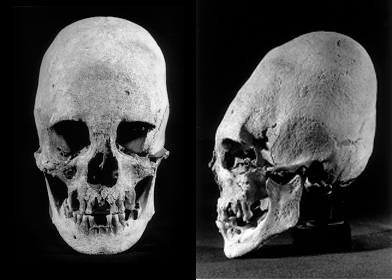
\includegraphics[width=0.70\linewidth]{chast-colebanie-osnov/alani/aw01.png}

\textit{Череп сарматской женщины.}
\end{center} 

Про Сарматов Аланов в популярной научной и околонаучной литературе зачастую умалчивается любопытная штука – некоторые найденные черепа Аланов и Аланок были сильно вытянуты назад (как у многих «каменных баб»). Ученые поясняют это «искусственной деформацией» без каких-либо оснований для такого утверждения. Просто решили, что у людей таких черепов быть не может, у всех должны быть, видите ли, головы более круглые.

А ведь потомки сих Аланок, тоже с вытянутыми головами, видны на портретах жителей Украины и окрестностей за 17-18 века. Тоже искусственная деформация?

Вытянутые, длинные черепа Аланов находят всюду, где обитала эта ветвь Сарматов – в нынешней Франции, Австрии, на Кавказе, Киевщине\footnote{Подобный череп обнаружен в 19 веке в кургане под Уманью, у фермы Марьянки. Однако захоронение относится ко времени, предшествующему Скифам и Сарматам, а также «трипольцам». Значит, люди с подобными черепами обитали на Киевщине с незапамятных времен.}. Археологи находят эти черепа и повторяют – искусственная деформация. 

%А ветвь аланов была большая и могучая, на много отростков – даже до Пакистана дотянулась, где поныне живет народ Калаш (Калаша). А может, калаши и не ветвь, а основа, кто знает? Хотя калашей осталось всего около 5000, они поныне сохраняют свои облик, обычаи и верования, отличные от соседних народов. Выглядят многие калаши своеобразно – я бы сказал, как славяне.

%Конечно, не у всех Аланов были вытянутые черепа, но кстати вытянутых и много, причем с остатками рыжеватых волос, нашел археолог Хулио Сесар Тельо в 1928 году в перуанской пустыне Паракас. И как обычно – сторонники инопланетной теории НЛО понимающе кивают головой, а ученые твердят об «искусственной деформации». 

А ведь довольно сравнить древние, гармонично сложенные вытянутые черепа и черепа в самом деле искусственно измененные, у разных африканских племен – огромная разница. Да и не только у африканских – во Франции этим занимались даже в 19 веке. Верно, подражали давним Аланам, для некоторых представителей которых такие черепа были прирожденной нормой.

Часть найденных в Европе вытянутых черепов археологи относят к Хуннам. Такие же черепа, только одни наука называет аланскими, другие – хуннскими. И про Хуннов тоже говорит – это искусственная деформация черепа! А когда по черепу воссоздают облик, то Хуннам рисуют узкие глаза – мол, монголоиды, а Аланам – пошире. Или лепят подобное из гипса.
 
Но меня занесло в сторону.

Пехоте Тавроскифов у Льва Диакона несколько противоречат конные Роксоланы у Тацита, ибо Тацит, говоря о Роксоланах как о народе, произошедшем от Сарматов (Rhoxolani, Sarmatica gens), описывает их как замечательных в конном бою, и беспомощных в пешем – так, по крайней мере, было, когда Роксоланы вторглись в Мисию во время Оттона и Вителлия. А по всем прикидкам Роксоланы и Тавроскифы один народ.

Но всё зависело от времени и места. Воевавшие с римлянами Сарматы были с головы до ног защищены кольчугой, в кольчуги же одевали и лошадей, покрывая глаза их продырявленными кружочками. Затем мы видим сарматских воительниц и воинов в кожаных латах с металлическими пластинами. Что до конницы, то если сведения Константина Багрянородного верны и Росы покупали лошадей у Печенегов, значит сами были в этом деле не очень-то. Может и Роксоланы – Росы, смешанные с Аланами – тоже не шибко делали ставку на конницу, хотя в летописях есть упоминания о ней, причем в непосредственной связи с князьями Вещим Олегом, Игорем и Святославом. 

Ученые относят Аланов к иранозычным. Это поспешный и слишком общий вывод, верный однако применительно к Аланам, обитавшим около Кавказа и смешавшимся с Иранцами. Но те Аланы, что жили по Днепру, были Славянами со славянским языком. Доказательство очень простое.

Мы знаем из летописей, что здесь жил славянский народ, именуемый Поляне. Довольно отбросить «п» и получить Оляне, те же Алане. Только так могло образоваться название «Роксоланы». Ибо Росы соединились с Аланами. А вспомним каневского Алана по имени Михей!

Более того, доводом для отождествления Аланов и Полян, помимо совмещения по месту и времени, служат былины. В них встречаются женщины-воительницы, именуемые «поляницы». На Украине это слово сохранилось в именовании пшеничного хлеба.

Былины порой освещают седые времена с фотографической точностью, беда лишь в том, что нынешние представления о седых временах совсем другие, и былинная правда воспринимается сказкой.

Верны былины в географии, они знают, например, киевскую речку Почайну под именем Пучайки или Пучай-реки. Былины же именуют Илью Муромца – казаком. Подобно Нартам, старинному богатырскому народу из преданий Осетинов, наши богатыри смотрят вдаль через подзорные трубы. Когда какой-нибудь богатырь приезжает, скажем, к черниговскому князю, тот спрашивает – ты коей земли, коей орды будешь?

Едет Добрыня Никитич в чистом полюшке, встречает поляницу удалую, Настасью дочь Никуличну, и лупит ее в голову\cite{gilder01}: 

\settowidth{\versewidth}{«Думала же, русскии комарики покусывают,} 
\begin{verse}[\versewidth]
На кони сидит же поляница, сворухнуласе\\
И назад же поляница оглянуласе,\\
Говорит же поляница да удалая:\\
«Думала же, русскии комарики покусывают,\\
Ажно русскии богатыри пощалкивают!».\\
Ухватила тут Добрыню за желты кудри,\\
Сдернула Добрынюшку с коня долой\\
А спустила тут Добрыню во глубок мешок,\\
А во тот мешок да тут во кожаной,\\
А повезе же ейный было добрый конь,\\
А повезе же он да по чисту полю.
\end{verse}

Далее конь разговаривает с поляницей – такие же говорящие лошади постоянны в преданиях Осетинов про Нартов.

Поляницы в былинах – не редкая диковинка, а постоянная героиня. Более того, в былине про Ставра сказано:

\settowidth{\versewidth}{Солнышко Владимир князь стольнё-киевской} 
\begin{verse}[\versewidth]
Солнышко Владимир князь стольнё-киевской\\
Задернул он почестный пир\\
На всих князей, на бояра,\\
На всих могучиих богатырей,\\
На всих поляниц да удалыих.\\
Соезжалися на почестный пир\\
Вси князи и вси бояра,\\
Вси могучии богатыри,\\
Вси поляницы удалыи.
\end{verse}

Знали сказители и Роксоланов – в былине «Соловей Будимирович» этот Соловей, вернувшись в Киев с моря Черного, призывает свою дружину – скидывайте с себя кожанки лосиные, надевайте кафтаны роскурлань-сукна! Былины помещают в наше Подолье некую Марью лебедь белую, подолянку да королевичну, русскую красавицу, по всем повадкам – сарматскую воительницу.

Всё найдется в былинах – распри со славянской тогда Литвой, странные отношения с Ордой, Батый (Батыга), какие как брались дани, какие одежды носились. Спелись в былинах исконно скифские и сарматские земли – Днепр и Дон, как небо отражается в реке, так в былине отразилось аланское прошлое Киевщины и язык старославянский, тот самый «церковный»\footnote{Александр Гильфердинг записал эту былину в Пудоге в 1871 году от крестьянина Никифора Прохорова, 51 года возраста, перенявшего былины от отца своего.}:

\settowidth{\versewidth}{А не стрели-тко ты меня Непры королевичной.} 
\begin{verse}[\versewidth]
Как тот ли этот князь стольне-киевской\\
А сделал он задернул свой почёстный пир.\\
Как вси-то к ему на пир собиралиси,\\
Вси там на пиру наедалися,\\
Как вси там на пиру напивалися,\\
Стали там оны вси пьянёшеньки,\\
А стали вси оны веселешенки,\\
Князи вси бояра-то русийскии,\\
А тыи-то могучи вси бог\'атыри,\\
Как вси-то они ведь там расхвастались.\\
Как тут была межу има\\
А тая эта Н\'епра королевична.\\
Как-то тая Непра королевична\\
Как говорит промолвит таково слово:\\
«А нету зде стрельцов добрых молодцов\\
Противо меня Непры королевичной!\\
Силою да нету ухваткою\\
Против стараго каз\'ака Ильи Муромца,\\
А красотою еще было угожеством\\
Противо ведь Михайлы П\'отыка Иванова,\\
А тишиною говорить смиреньицом\\
Противо Добрынюшки Микитица,\\
А нету-то видь еще богачеством\\
Против-то ведь Дюка Степанова,\\
А нету-то да ведь смелостью\\
Противо смелаго Алешеньки Поповича,\\
Поступкой походкою пощапкою\footnote{Щегольство.}\\
Противо-то Чурилки щапа Плёнкова».\\
Сама она еще не спохвалила\\
А тихаго ведь Дона-то сына Иванова,\\
А своёго-то мужа любимого.\\
Как тихий тут Дон сын Иванович \\
А говорит промолвит таково слово:\\
«Ай же ты да Непра королевична!\\
Когда же ты охвоча-то была удалая\\
Стрелять-то было стрелочок каленыих,\\
Пойдём-ко мы с тобой на чисто поле,\\
Станем стрелять стрелочок каленыих,\\
Который ведь стрелять видняе-то?»\\
Как тут-то тая Непра королевична\\
Взимет тут-то ножичок булатныи,\\
Как тое-то колечушко серебряно,\\
Относит что за версту за мерную,\\
Натянула тут она свой да тугой лук\\
А клала ёна стрелочку каленую,\\
Стрелила тут за версту за мерную,\\
Попадала в колечко-то серебряно,\\
И росколола ёна стрелочку равным равно,\\
Да равным то равно стрелку на двое.\\
А клали половинки на весы они,\\
Никоя никоёй не перетягивать.\\
Как тихий тут Дон сын Иванович,\\
Розгорелось ёго сердце богатырское,\\
Как скоро натянул свой он тугой лук,\\
Кладывает стрелочку каленую.\\
Как начал тут Дон сын Иванович.\\
Начал он стрелочкой помахивать\\
А начал ведь-то сам выговаривать:\\
«Ай же ты моя любима калена стрела!\\
Пади же ты не на воду, не на землю,\\
А ты пади ко Непры королевичной,\\
А ты пади же ей во белую грудь».\\
Как тут-то тая Непра королевична\\
Как тут-то ведь она да прослезиласи\\
А тут-то ведь она порасплакалась:\\
«Ах тихий ты Дон сын Иванович!\\
А не стрели-тко ты меня Непры королевичной.\\
Да несу я ти сына любимого,\\
А по колен-то ноженьки во серебри,\\
А по локоть-то рученьки во золоти,\\
А по косицам текут будто звездышки,\\
На зади-то возсият будто светел месяц,\\
Впереди-то как будто солнышко».\\
Как розгорелось ёго сердце богатырское,\\
А ничего тут он ведь не последовал.\\
Как скоро он стрелил ю во белую грудь,\\
Как пала тут она на сыру землю,\\
Облилась она кровью тут горючею.\\
Как тихий тут Дон сын Иванович\\
Взимает он ножищо тут кинжалищо, – \\
Ино ль то ведь еще правда ль есть?\\
Пластал-то он ведь ей да белую грудь.\\
Как было-то ведь тут да до правды бы:\\
Засиян-то ведь во чреви тот сын-то был,\\
По колен-то ноженьки во с\'еребри,\\
По лок\'оть-то рученьки во золоти,\\
Назади просвичать будто свитёл месяц,\\
Впереди еще как там солнышко.\\
Как взял это ножищо он кинжалищо,\\
Становил он-то ножик ведь супротив себя,\\
А становил он ножик, выговаривал:\\
«Да куды пала головка белой лебеди,\\
А тут пади головушка сера гуся».\\
Пал он на ножищо тут кинжалищо,\\
Да тут-то им пришла е горьк\'ая смерть.\\
Как от их-то от крови от крестьянскии\footnote{Христианской.},\\
От крестьянскии крови безнапрасныи,\\
Как протекала тут да Непра река.\\
В глубину река двадцати сажон,\\
А в ширину река сороки сажен.\\
Только-то ведь Донушку славу поют,\\
А той ли этой Непры королевичной.\\
Тут-то их да жительство решилоси.\\
\end{verse}

И складывались эти былины да во времечко, когда Сарматы, коих всех ученые объявили «ираноязычными племенами» и отодвинули далеко в прошлое, говорили одним языком с нашими богатырями, сиживали с ними за одним столом, и были если не всем здешним народом, то доброй его половиной. И если «поляница» – это Аланка, то былинный казак – это «ас» или «аз», такой же Алан. Поныне в Ближних пещерах лежат останки, приписываемые «старому казаку» Илье Муромцу.

Это странные останки. Их ведь изучали, во время Перестройки, и пришли к выводу, что Илья вообще не мог ходить из-за некоего заболевания позвоночника (я не мог найти подробности). Рост Муромца был 177 сантиметров. Необычно толстые кости черепа – лобные, теменные, затылочные. Выдержат, по словам проводившего исследование судмедэксперта Сергея Никитина, удар молотком, от которого у другого человека будет черепно-мозговая травма, вдавленный перелом.

Такие же необыкновенно большие и кисти рук. Более мощные запястья и ключицы.

Всё это некоторые ученые списывают на болезнь. Кроме того, хотя по былинам Илья и просидел сиднем 33 года, но потом в подвижности давал фору многим, значит таки ходил. Почему бы не предположить, что Илья просто отличался от людей обычного биологического вида? Возможно, такое строение тела было для богатырей нормой? Не от болести у Илюши крепки костушки, а богатырское строение таковское. Настоящая боевая машина. Думаю, у других богатырей было подобное.

Муромец скончался в возрасте 40-45 лет. При осмотре останков, у него обнаружено несколько переломов ребер, правой ключицы, проникающее ранение левой руки, сквозное ранение грудной клетки острым предметом – предполагают, от сего и помер.

Что же, вдоволь наговорившись про Аланов – но я к ним еще вернусь – приступлю к тому, что послужило заделом главы – городам Амадоку и Азагориуму. Памятуя о разных народах, скифских да сарматских, сможем более толково рассмотреть птолемееву карту, точнее ее кусок. 

Правильнее говорить, однако, «карта по Птолемею». Клавдий Птолемей был математиком, астрономом, астрологом, географом из Александрии, что в Египте. Общепринято считать, будто Птолемей жил в первом веке нашей эры, хотя труды его известны Арабам только вроде бы с девятого века, а основная его работа по географии – собственно «География» – всплывает в Италии почему-то лишь в начале 15 века и в латинском переводе, хотя по источникам (я не проверял) греческие списки прослеживаются с 13 века. Веком ранее начинают прослеживаться опять же латинские переводы другого сочинения Птолемея, астрономического «Альмагеста», причем выполненные с арабского. 

Выходит, что две известнейшие работы Птолемея стали известны посмертно спустя почти десять веков после их написания, если придерживаться традиционной хронологии, в которой возможны любые чудеса. Более правдоподобным мне кажется, что возникновение списков (прослеживаемых по источникам) с этих работ и есть примерное время написания подлинников. И Птолемей жил незадолго (в пределах нескольких веков) до пришествия на Киевщину Вещего Олега.

Карты, нарисованные рукой Птолемея, не сохранились. Ныне известны лишь составленные «по Птолемею», и я буду использовать карту из рукописного издания 1480 года, так называемого «Уилтонского кодекса».

Немного о самой «Географии». В основу своего труда Птолемей взял работу Марина из Тира (Μαρίνος ο Τύριος), которая не дошла до нас. Другое упоминание Марина встречаем только у арабского географа аль Масуди, который отзывался о картах Марина как о превосходящих карты Птолемея. Правда, сам Птолемей говорит, что Марин карту начертить не успел, а оставил только текстовое описание.

Именно Марин первым из известных нам картографов ввел координатную систему по ширине и долготе. Единицами измерения в ней ввел градусы, а с одним градусом соотнес примерно 500 стадий. По странам составлялись списки городов, городам назначались координаты. Потом, исходя из этих текстовых описаний и уточняя положение по определенным формулам, следовало чертить карту, причем надо было сферическую поверхность (Греки знали, что Земля круглая) перенести на плоскую.

Но Птолемей пишет, что по данным Марина верную карту начертить невозможно, вдобавок Марин дает не\-полные координаты – то приводит одни лишь широты, то долготы. «География» Птолемея, таким образом, это надстройка над работой Марина, с многочисленными исправлениями и дополнениями (из других источников), которые позволяют таки начертить по текстовому описанию приемлемую плоскую карту. 

Но многие города так и остались с «одной координатой». По карте видно, что знаменитые Амадок и Азагориум, а ниже Сарон и Ниоссон, лежат на одной долготе. Подобные «однодолготные» города есть и восточнее вдоль Хипаниса.

Возникает вопрос, а как же заданы координаты рек? Ведь река – не единичная точка на карте, но совокупность точек. Если записывать такую последовательность точек, составляющих реку, то, допустим, через определенные промежутки. И затем, перенеся эти точки на карту, соединить их линией. Так мы получим примерные очертания реки.

Однако «География» Птолемея не содержит таких данных по рекам. Даются сведения, что река такая-то протекает в такой-то местности. И указаны координаты ее устья и, если известны – истока. Следовательно, реки на картах, составленных по Птолемею, изображены условно от точки истока до точки устья.

«Дополненные» координаты для Азагориума и Амадока – хотя я не исключаю, что они в самом деле лежали на одной долготе – и примерные изображения рек на карте Птолемея не дают представления о том, на каком берегу находились эти города и даже как далеко они отстояли от берега.

Вот города по берегам Днепра из труда Птолемея:

\begin{longtable}{l|l}
Город & Координаты\\ \hline
Азагорион (Азаргариан) & 56° 30'  50° 40'\\
Амадока & 56°(30') 50° 30'\\
Сарон & 56° 50° 15' (45')\\
Серимон & 57° 50°\\
Метрополис & 56° 30' 49° 30'\\
Олбия (Борисфенис) & 57° 49°\\
\end{longtable}

%Город & Координаты\\% \hline
%Азагорион (Азаргариан) 56° 30'  50° 40'\\
%Амадока 56°(30') 50° 30'\\
%Сарон 56° 50° 15' (45')\\
%Серимон 57° 50°\\
%Метрополис 56° 30' 49° 30'\\
%Олбия (Борисфенис) 57° 49°\\

Можно ли перевести их координаты в одну из используемых ныне картографических проекций? Ученые занимаются этим давно и приходят к противоречивым выводам.

Кроме координат городов, Птолемей дает примерные координаты гор (в качестве единичных точек) и описывает, где какие народы живут – основываясь невесть на чьих данных.%Роксоланы у Птолемея помещены на берег Азовского моря, а севернее их – Амаксобии и Аланы.

Давайте наконец поглядим на карту, памятуя, что ее начертил не Птолемей. Она составлена кем-то по текстовому описанию, сделанному Птолемеем, что приводил координаты, рассказывал, какие где живут народы и так далее. Порассуждаем над картой, хотя вернее было бы рассуждать над текстом Птолемея. Карта всё же нагляднее, но искажена переосмыслением составителя карты. 

\begin{center}
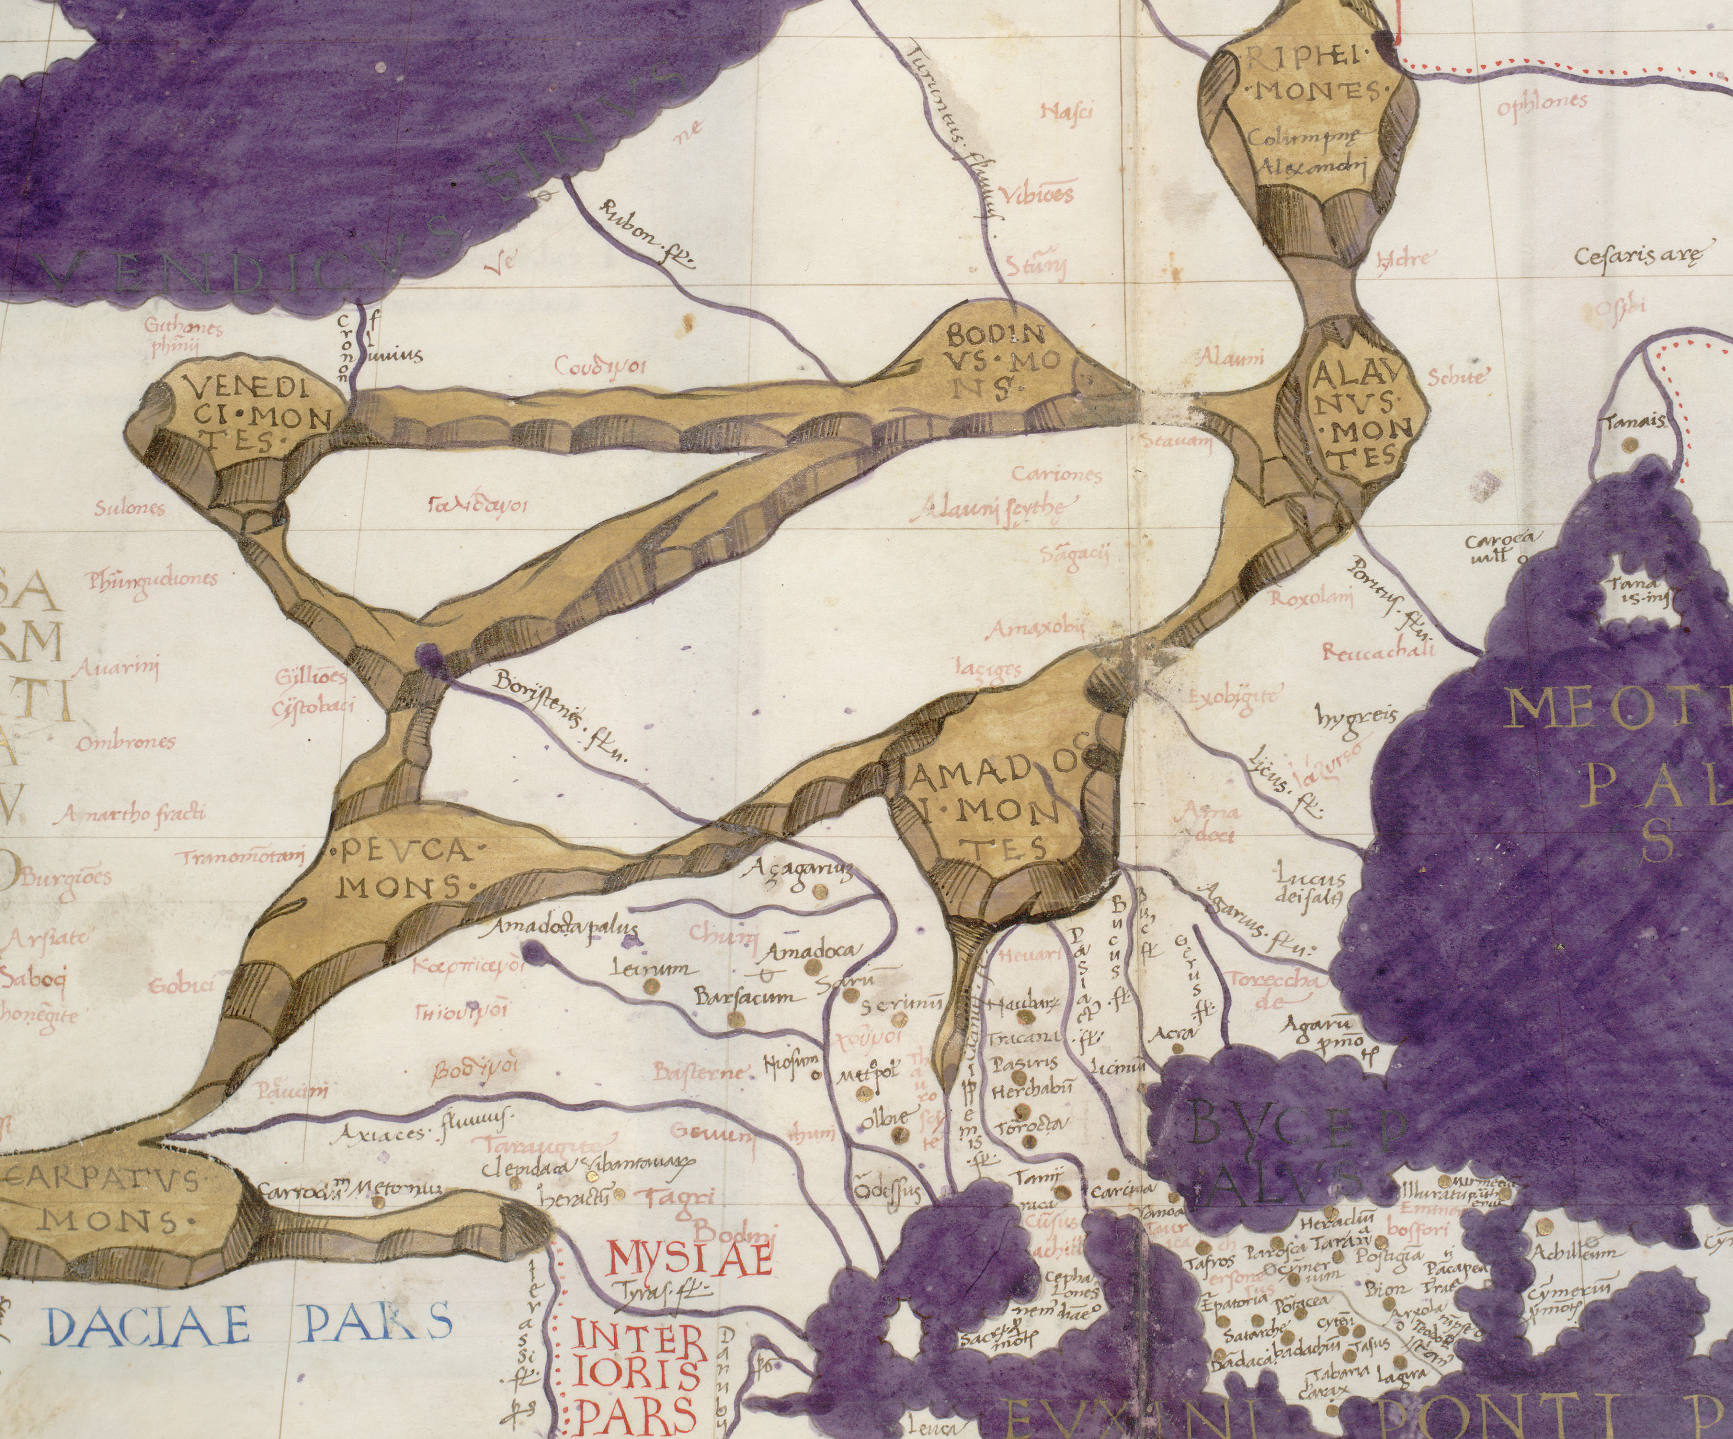
\includegraphics[width=\linewidth]{chast-colebanie-osnov/alani/ptol.jpg}
\end{center}

Многие исследователи не видят разницы между сочинением Птолемея и «его» картами, строя на основе последних умозаключения. В то время как сии карты могут служить лишь для поверхностного суждения о сведениях, изложенных Птолемеем. Таким ли будет суждение собственное, вынесенное при близком знакомстве с «Географией»?  

Сразу бросается в глаза, что карта ориентирована не на привычный нам север, а со смещением, как если бы взять современную карту и повернуть ее против часовой стрелки. А ведь Греки отлично разбирались в сторонах света. Здесь карта не просто от фонаря нарисована, но с координатной сеткой, где меридианы (параллельные линии, от нулевой из которых отсчитываются долготы) ведут к полюсам.

Выходит, что полюса на картах, составленных по Птолемею, отличны от современных нам. Я не буду здесь делать из этого выводы. Но далее, пользуясь сторонами света в разговоре об этой карте, применяю ту систему координат и те полюса, которые присущи именно этой карте.

В правом верхнем углу – устье Tanais, Дона. Он впадает в Азовское море (Мэотийское озеро).

Левее – Alanus Montes, Аланские горы. 

Горная цепь тянется от Аланских гор вниз-налево к Amadok Montes, горам Амадок. Это примерно холмы вдоль Северского Донца, Донецкий кряж.

К северу от них на карте подписаны местные народы – кроме прочих Аланы Скифы, Амаксобии\footnote{Корень «άμαξό», амаксо, значит «правящий повозкой».}.

Но пространство западнее, левее этих народов – пусто. Населено ли оно ими, или нет – неясно. От гор Амадок горная цепь идет дальше налево, как понимаю, как запад, и пересекает наш Днепр – на карте обозначен как Борисфен, Borisfenis flu.

Ниже пересечения Днепра горами, первым, на правому берегу, идет город Азагориум. Ниже, через некую реку – город Амадока. По левому берегу южнее – Сару.

Ниже Сары, в Днепр с правого берега вливается некий приток, берущий начало в озере Амадок. По его левому берегу лежат города Лемум и Барсакум. Южнее устья сего притока расположен город Ниосум.

По левому берегу Днепра далее – город Метрополь, затем Днепр раздваивается, впадает в Черное море, и между устьями Днепра видно «Одэссус». Этот Метрополь, невзирая на координаты, некоторые ученые соотносят с Киевом. Ольвия помещена к востоку от второго рукава, весьма глубоко в материке.

Также на карте есть горы Бодинов (небось геродотовы Будины). А возле Аланских гор живут Аланы. Горы Амадоков и город Амадока явно связаны. Можно предположить существование одноименного народа – Амадоков. Так и есть – они показаны южнее гор Амадок. От города Амадоки этих Амадоков отделяют горы.

Местность возле Азагориума и Амадоки, по карте, населяют Кхуни – и сложно усмотреть в этом нечто иное, нежели Хуннов или Гуннов. А ведь наука говорит, что Птолемей жил в первом веке нашей эры! И эта же наука говорит, что Хунны проявили себя в пятом веке, во всяком случае тогда они попали в Европу! Что же, по общепринятой науке, Птолемей – великий провидец? Нет, это еще одно подтверждение ошибочности хронологии, которой придерживаются ученые.

Я попробовал умозрительно наложить карту по Птолемею на современную, учитывая, что каждая горная цепь на древней карте была задана точкой, и по неким соображениям дорисована. Над Азовским морем получаются горы Аланские и Амадокские. Это возможно современный Донецкий кряж, проходящий между Луганском и Донецком и затем сворачивающий (при современном полюсе) на юго-запад к Мариуполю и оттуда еще западнее, почти к излучине Днепра ниже Запорожья.

На карте по Птолемею мы видим, что некая возвышенность, горный рукав, пересекает Борисфен и тянется к горам Певка, к югу от которых лежит озеро Амадок (Amadoc palus).

Попытаемся пробить Певку и Амадок по древним источникам. Не горы, но остров Певка и народ Певкины помещаются Греками в устье Дуная. Название острова в переводе значит Сосновый от растущих на нем сосен. По Страбону, населяющие его Певкины произошли от народа Бастарнов. Остров сей был известен еще во времена Александра Македонского. Арриан в «Походе Александра» упоминает крутые берега острова, а вдоль – речной рукав с течением столь сильным, что невозможно стать на якорь.

Ныне в устье Дуная нет ни огромного острова с остатками города, ни стремительного рукава. Напротив устья, в море, находятся жалкие остатки большого некогда острова с похожим на Певку именем – Левка, он же остров Ахилла, теперь его величают Змеиным.

Теперь про Амадоков. Ничего про них, кроме географических названий вроде гор Амадоков, города Амадоки, озера Амадоки я не нашел.

Зачем всё это, если, казалось бы, Птолемеем даны координаты, бери да переводи в современные. Но это тупиковый вариант, ибо поныне неясно, как именно переводить. Этим занимается множество исследователей, и у них выходит разное. И нигде в известных мне попытках такого перевода не учитывается иное положение полюсов. 

А я не обладаю достаточными знаниями, чтобы взяться за дело, но даже если бы мне удалось совершить точный, а не умозрительный перенос карты Птолемея (во многом весьма условной) в какую-нибудь современную проекцию, что бы я получил? Мне нужно, во-первых, русло Днепра. У Птолемея русло задано начальной и конечной точкой. Координаты городов Амадоки и Азагориума с их одинаковой долготой вызывают у меня подозрение. 

Так что за возвышенность или горная цепь между горами Певка и Амадоки, пересекающая Днепр? Подобное пересечение ныне известно лишь в месте затопленных порогов около Запорожья. Исходя из этого, Амадока и Азагориум лежат тоже ниже порогов, а никак не на Киевщине. В древних источниках нигде, кроме «Географии» Птолемея, эти два города не упомянуты.

Если горы Амадок это Донецкая возвышенность, то западнее ее лежит Приазовская возвышенность, что несколько уходит от порогов южнее. А горами Певка могут быть холмы к западу и северу от Кировограда.

Одним словом, если возвышенность через Днепр на карте по Птолемею не выдумка, то ее придется пояснить одним – изменением рельефа местности. Например, горная гряда была занесены слоем грунта таким образом, что превратилась почти в равнину.

Что до Киевщины, Полтавщины и Черниговщины, то они на карте по Птолемею лежат в пустом месте между вышеупомянутой загадочной возвышенностью через Днепр и следующей возвышенностью к северу, возможно Валдайской, где начинается Днепр. И Птолемей не знает там ничего, кроме «пустыни», в которой живут Скифы Аланы и несколько других народов.

А может статься, это всё другие горы, сгинувшие, и сопоставление с современными возвышенностями – ошибочно. Ведь не существует более огромного озера Амадоки, которое упорно держалось веками на множестве старинных карт.

Теперь отрешимся от того, что нарисовано на карте. Это не карта Птолемея, но составлена по тексту его «Географии». 

Сравниваю с текстом. Данные, перенесенные на карту, приведены в третьей книге, главе пятой. Всё это, по Птолемею – Сарматия. Он пишет, в параграфе 19, что по всему берегу Мэотиды живут Иазыги (Ιαζυγες) и Роксоланы (Ρωξολανοι). А за ними, вглубь страны – Амаксобии (Αμαξοβιοι) и Аланы Скифы (Αλαυνοι Σκυθαι). Описание места их жительства размыто, однако по нашим летописям, тоже размытым, примерно те места населяли Поляне, славянский народ. Они же, выходит, те, кто у Птолемея – Аланы, скифский народ. 

Однако Языги (Ассы) считаются другим названием Аланов. Может, прав Птолемей, разделяя их. А может, перечень народонаселения в «Географии» сводный, туда выписывались данные из разных источников, а составитель по неведению не сопоставил Ассов с Языгами и поместил их как два отдельных народа.

Аланы неразрывно связаны с рекой Борисфен – в поэме римского императора Адриана приведено имя коня Юлия Цезаря – Борисфен Аланский.

Что же случилось с Аланами? Они растворились в населении одних мест и составили основу населения других. На Киевщине Поляне-Алане – проживали до прихода Вещего Олега с Русами и неясно, в какой степени произошло смешивание, а с учетом многочисленных разорений Киева да окрестностей, и последующих волн заселения, можно предположить, что в некоторых современных киевлянах есть доля аланской крови, однако никто не является Аланом полностью. 

От Аланов остались также названия стран и местностей, где они проживали – при этом сами Аланы могли, опять же, сгинуть оттуда или раствориться, либо растворить. 

Земли Польши в давнее время звались Полонией, а на старинных картах между Полонией и Молдавией лежит Руссия (не Киевская Русь и не Московия), а севернее Руссии – Волиния, в чьем имени тоже угадывается аланское созвучие. Также и другие Аланы – Асы, Язы, Осы – оставили след свой в Осетии, Азербайджане, в имени Азовского моря, возможно и современной Албании. Примечательно, что на родном языке Шотландцев – гаэльском – Шотландия называется Алба или Албания. А Scotland она называется от Ск\'отов (Скоттов) – ряд давних источников возводит название к Скоте, дочери фараона Сингриса, современнице Моисея и жене предводителя некоего возможно скифского народа, который двинулся затем из Египта и, после скитаний, осел в Ирландии. Кстати в нынешней Шотландии существует местность под названием Росс.

Но это уже о Росах, про них мы поговорим позже, они ускользают, тоже всюду оставляя свои следы, причем даже в Азии, Малой и обычной. Да и Скифы.

В устье Иордана лежит город Beit Shean (Бейт Шеан), где туристам показывают развалины древнего города – остатки зданий с колоннами, громадного амфитеатра на 7 тысяч зрителей, бассейнов, общественных бань. Это прежний город Скифов, Скифополис, дважды упомянутый еще в Ветхом Завете. Один раз – когда после странствий по пустыне, сыны Израилевы начинают уничтожать или подчинять себе города. Второй раз о Скифополисе сказано в Книге Иудифь. В ней же, Олоферн – военачальник Ассирийского царя Навуходоносора – «разграбил всех сынов Рассиса», перемещаясь где-то возле Киликии.

А возьмите название другого города – Иерусалим, в давних источниках именуемый Русалим и Урусалим. Я не поднимаю тут тему возможного родства Славян и некоторых Евреев – хотя можно почитать работы Пола Векслера, например «Ашкеназийские евреи: славянско-тюркский народ в поисках еврейской идентификации» (Paul Wexler The Ashkenazic Jews: A Slavo-Turkic People in Search of a Jewish Identity). Другие исследователи напротив, выводят русских от восточных Евреев, плохо понимая вообще, что значит понятие «русские» (прилагательное, применяемое к народам, попавшим под власть народа, известного как Росы), третьи стараются их всеми силами противопоставить.

Можно взять название любого города и прилагать его то к одному, то к другому. Русалим – еще к русалкам близко, и к русальим дням, русалиям.

Вот Скифополис – более твердая почва для размышлений. Город Скифов. Город в выгодном торговом месте – устье Иордана. Сам по себе, если бы окружающее население было к Скифам враждебно, он бы не возник. Не выстояли бы Скифы. Значит, в том месте, в некоторое время, Скифы могли считаться если не «своими», то дружественными. Возникает вопрос – не было ли среди тамошнего окрестного населения других Скифов? Каково было самоназвание Скифов, населявших Скифополис?

О Скифах в Азии пишет Геродот, касаясь истории Мидийского царства. Сменили один другого три правителя – Дейок, Фраорт, Киаксар. Последний расширил границы владений, покорив Ассирийцев. В это время в Азию явилось войско Скифов, которые гнали Киммерийцев из Европы. Во главе войска стоял царь Скифов по имени Мадий (возможно, Матий – от «мать», так же как Батий – от «батя»), сын Протория. Мидяне пытались дать Скифам отпор, но проиграли – не только в сражении, но и во властвовании над Азией, и Скифы держали последнюю в своих руках еще 28 лет.

После битвы с Мидянами Скифы двинулись на запад, в Палестинскую Сирию, но были остановлены египетским царем Псамметихом, который лично вышел к ним с дарами и договорился про обход его земель. Скифы отправились через и ныне существующий древний город Аскалон, и по некой причине не тронули его. Последующие три десятилетия Скифы брали дани с азийских народов, и грабили их помимо даней, но постепенно были перебиты Мидянами. Те отвоевали некогда подчиненные себе земли назад, кроме оставшегося независимым от них ассирийского Вавилона. Будущий поход персидского царя Дария против Скифов (когда в помощь Скифам пришли Савроматы, Гелоны и Будины) был вызван желанием отомстить за столь длительное былое господство над Персами (Иранцами).

Но может, Скифы или родственный им народ обитали в Азии еще до преследования Киммерийцев?

Посмотрим на карту. Какая страна находилась неподалеку от Скифополиса? Финикия\footnote{Отметим сходство ее названия с Венецией.}. Все ученые знают, кем были финикийцы – семиты, изобрели вдруг свою азбуку, потом ее переняли и расширили Греки, а Кирилл и Мефодий на досуге положили азбуку Греков в основу славянской.

Мне кажется, дело было наоборот. У неких изначальных Скифов и Сарматов был свой алфавит. Они жили, кроме прочего, и в Азии. Финикийцы – ветвь этих Скифов либо Сарматов, мне трудно их различать. Славяне – тоже ветвь Скифов и Сарматов. Поэтому алфавиты Славян и Финикийцев подобны. А Греки?

Проще ответить, если записать Греков в потомков Скифов и Сарматов. В Греции раньше жил народ Пеласги (Πελασγοί). Геродот отмечал, что говорили они на варварском языке. Эллины – на греческом, а вот Пеласги – на варварском. Варварами для Эллинов обычно были Скифы.

Пеласги соединились с Эллинами и другими народами, в том числе темнокожими (о чем свидетельствуют многочисленные монеты и рисунки на посуде\footnote{Судя по тем же рисункам, в давнее время люди сосуществовали с Сатирами, Кентаврами и другими существами, которых наука считает сказочными.}) – так возникли Греки, говорящие на языке Эллинов. Но если Пеласги являлись частью Скифо-Сарматского народа, общности, то понятно, почему у Греков такой же алфавит, как у Славян или у Финикийцев.

А если переплыть из Греции на восток, мы попадем к бывшей Финикии, а также в Палестину. Палестиной эта страна называется от некогда жившего там народа, известного древним Евреям как «Пелистим» (библейские язычники-Филистимляне)\footnote{Про них много рассказано в Ветхом Завете. Например, в Книге Царств, Фелистимляне отобрали у сынов Израиля ковчег со скрижалями, и принялись возить оный по своим городам, никто не хотел у себя его оставлять, ибо местное население покрывалось «болезненными наростами».}. Не надо далеко ходить, чтобы усмотреть общую основу у Пеласгов и Пелистима. Они жили и в Греции, и в Палестине. Кто в каком направлении переселялся – дело стороннее.

Город Скифополис находился там, где обитали ветхозаветные Филистимляне.

Всюду Славяне, что ли? Почти. Некий большой народ с более-менее одинаковым языком (отличавшийся говорами) в давнее время населял, кроме прочих народов, Европу и Азию. Части этого народа именовались, в разное время, в разных местах – Скифами, Сарматами, Пеласгами, Славянами, Полянами, Аланами, Асами, вероятно и Хуннами, Готфами – а части всё дробились, какие-то сохраняли величину и язык, какие-то утрачивали общность с родственным народами, роднясь с другими.

Стремление ученых превратить эти, скажем так, славянские народности, в дикарей доходит до крайности. Письменности их лишили, лишают и ювелирного искусства. 

Всем известно про «золото Скифов» – золотые украшения, равных которым трудно сыскать и поныне. Их отличительные черты – определенный стиль, названный «скифским», насыщенность бытовыми сценами, животными, да сюжетами якобы из мифологии Греков. Наука утверждает – Скифы заказывали вещи из золота у Греков. Мол, только Греки были мастерами в этом деле!
  
Найдут в скифском кургане золотые кругляши с портретами – говорят, что это не монеты, но бляхи. Вестимо, зачем «диким» Скифам монеты? А что значит «бляхи», каково их предназначение – между пальцами крутить? Не понимаю. Бляхи. 

Или отыщут шлем и называют его «греческим», хотя точно в таких же шлемах Скифы представлены на древнем литье. Почему женщин со скифских изображений ученые именуют «юношами»? Животных же вроде гриффонов, которые показаны рядом с лошадьми, львами, зайцами и утками считают выдумкой. Стороной обходят и постоянный образ сфинкса в скифских украшениях.

%В Керчи рядом с жилыми домами на улице Братьев Перепелицы находятся остатки кургана – поросший травой долгий пригорок, в котором в конце 19 века нашли выложенный каменными плитами «склеп Деметры», искуссно расписанный фресками. В 1942 году его повердил взрывом гранаты немецкий зольдат. Возведение в 1970-х жилого квартала ухудшило состояние склепа, его стало затапливать грунтовыми водами. Веками стоял посередине погребальной камеры деревянный гроб с останками – всё это разрушилось, едва лишь вытащили его на поверхность.

Ювелирные произведения Скифов донесли до нас и других, помимо гриффонов, неведомых ныне существ, как например эти кошкоподобные звери с пастями, состоящими словно из лепестков, служащих вероятно для заталкивания пищи в рот. Поскольку этот образ повторяется, предположу, что он передает животных, с которыми Скифы так или иначе соприкоснулись.

Поглядим на «кошек»\footnote{Картинки далее – из книги М. И. Артамонова «Сокровища скифских курганов в собрании Государственного Эрмитажа», 1966.}.

\vspace*{\fill}
\begin{center}
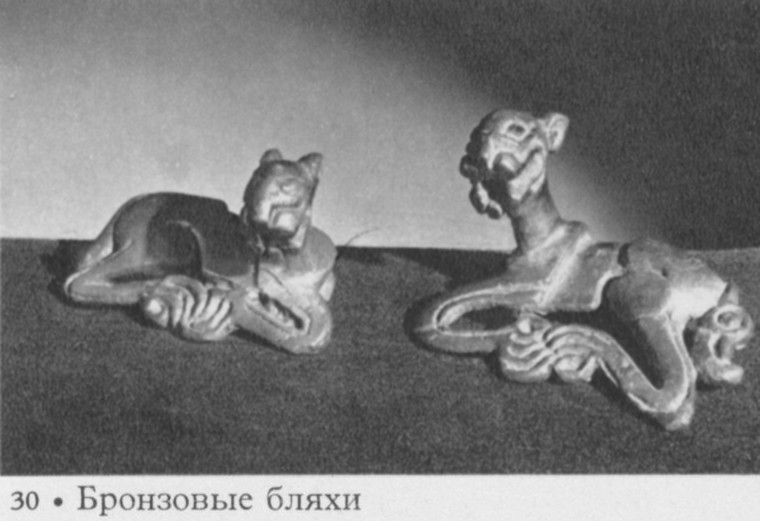
\includegraphics[width=\linewidth]{chast-colebanie-osnov/alani/artamonov-mi-1966-030.jpg}
\end{center}
\vspace*{\fill}
\newpage
\vspace*{\fill}
\begin{center}
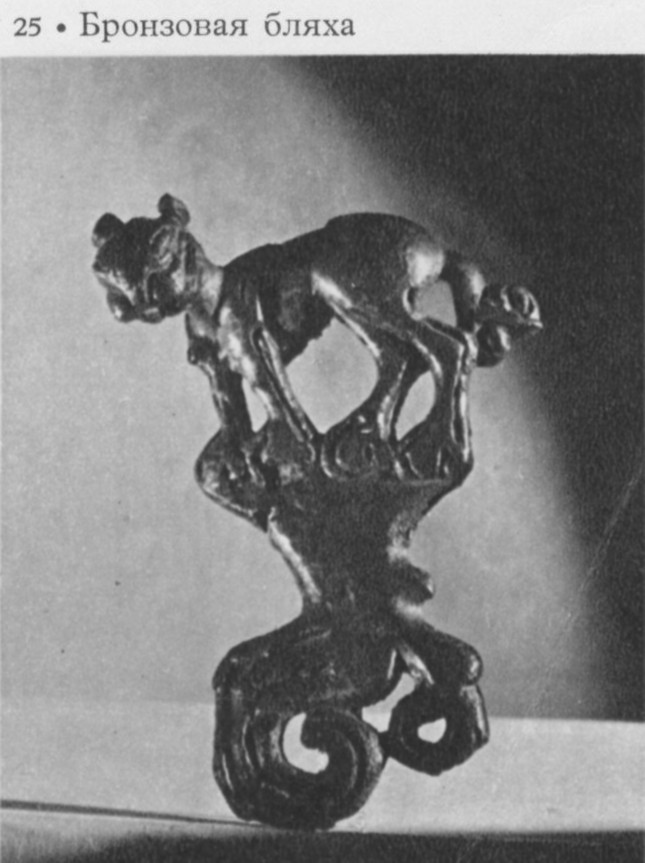
\includegraphics[width=\linewidth]{chast-colebanie-osnov/alani/artamonov-mi-1966-025.jpg}
\end{center}
\vspace*{\fill}
\newpage

А вот скифский золотой гребень из кургана Чертомлык, вид с одной и другой стороны.

\begin{center}
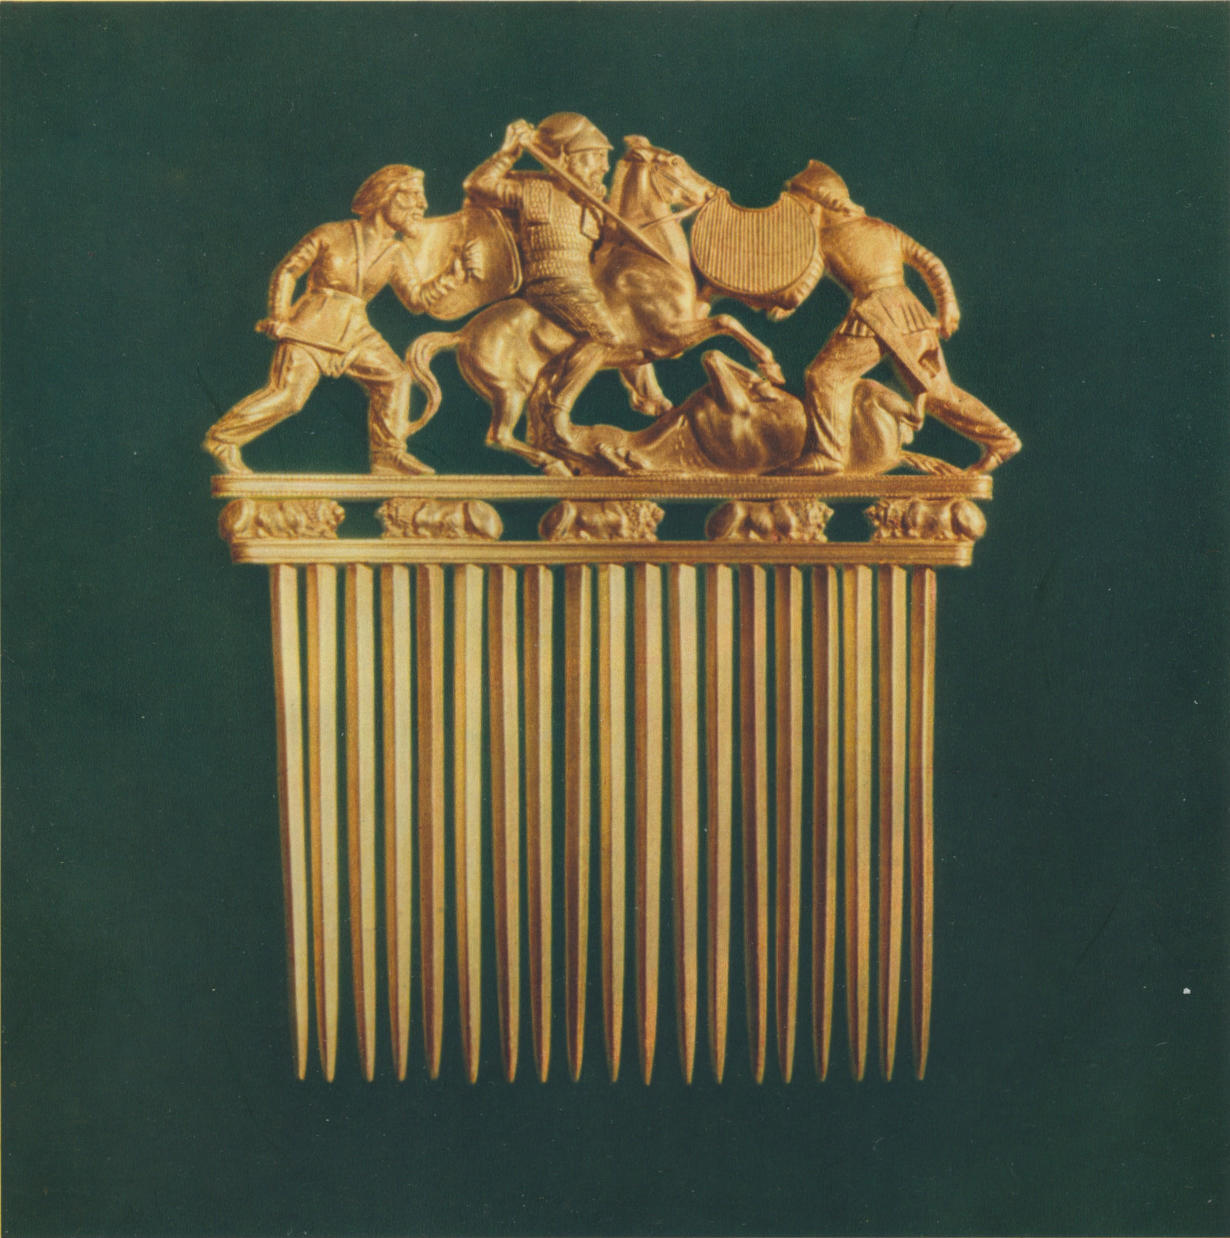
\includegraphics[width=0.75\linewidth]{chast-colebanie-osnov/alani/greben01.jpg}
\end{center}


\begin{center}
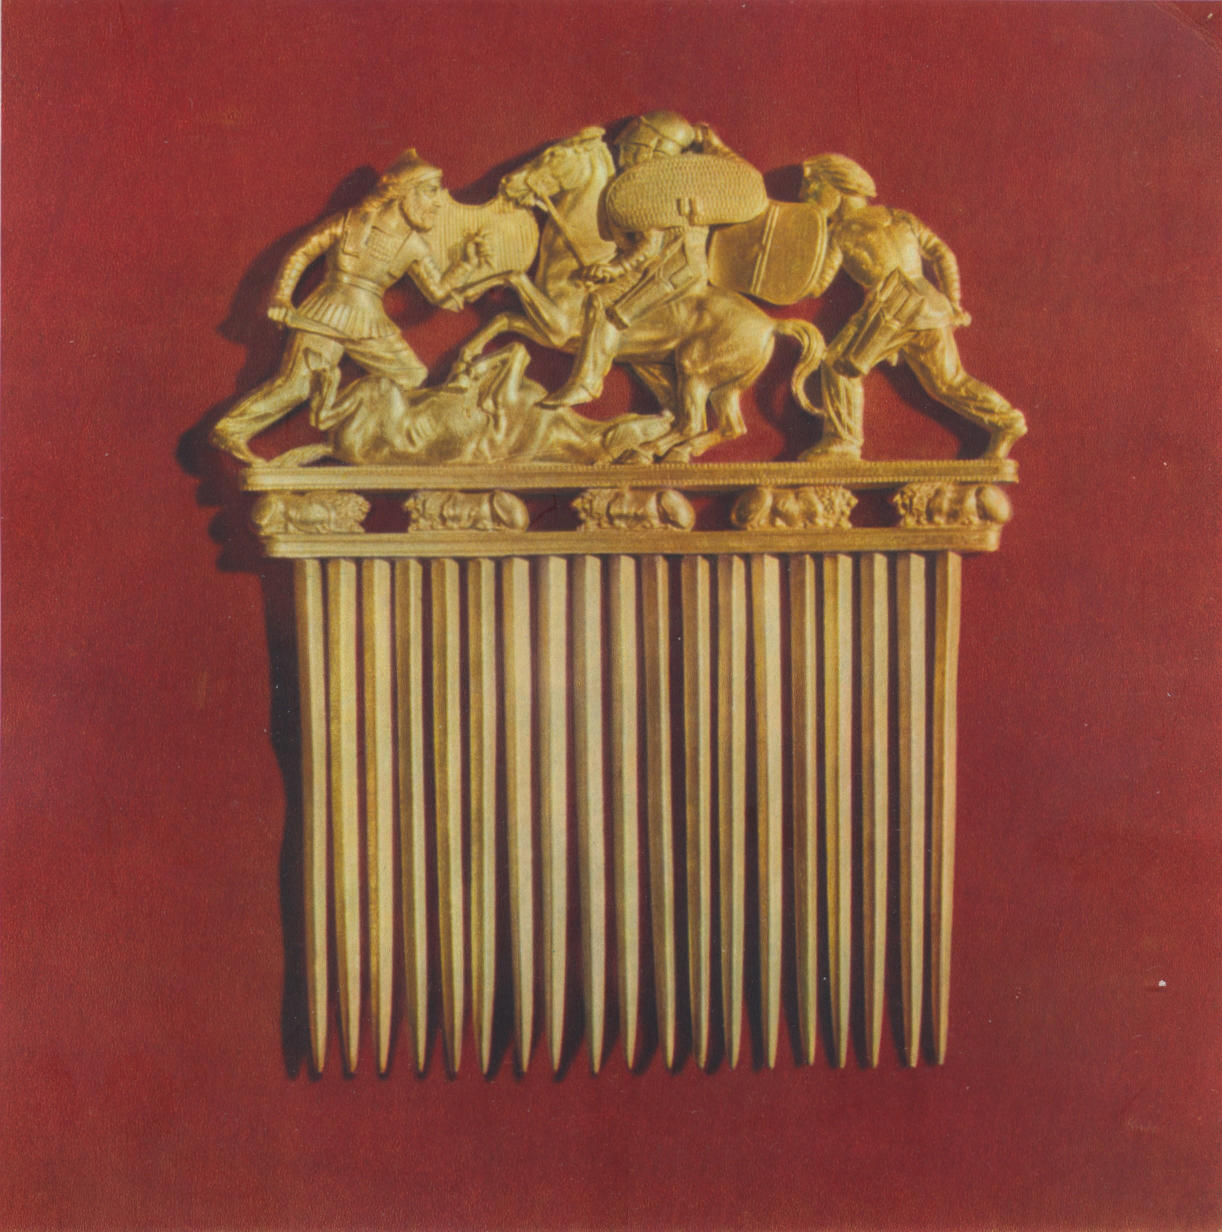
\includegraphics[width=0.75\linewidth]{chast-colebanie-osnov/alani/greben02.jpg}
\end{center}

Обратите внимание на всадника и лошадь. Судя по этому и множеству других изображений, Скифы редко пользовались сёдлами, а кони их были довольно низкорослыми, размером как нынче в Исландии. Кажется, и у других народов такие лошадки в старину были более распространены, о чем свидетельствует искусство. А на рельефах колонны Траяна в Риме, сарматская конница тоже предстают перед нами бесседельной да лишенной шпор.

Седла и стремена появились в землях Украины, вероятно, для удобства не столь умелых, как местные, наездников, коими были пришлые Русы.  Вспомним – они, поселившись с Вещим Олегом в Киеве, покупали лошадей у Печенегов. К этому относится и упомянутый Львом Диаконом упор на пехоту у святославовых Тавроскифов. А быть может, причина иная – другая привычка верховой езды. Кстати, шпоры впервые среди Славян начинают встречаться у прежнего, славянского населения нынешней Австрии только в 8 веке нашей эры, как следует из найденных погребений. 

Вещий Олег, Русы? Исследователи, склонные видеть в них скандинавов, встрепенулись и справедливо могут заметить, что скандинавы таки предпочитали сражаться пешими.

Что же, поговорим о скандинавах.

%Развернем карту, поглядим названия городов Австрии. По большому счету она протиснулась на запад между славянсикми странами, Чехией да Словенией. Так, Алланд. Понятно, от Аланов. Что еще? Еще не совсем онемеченные Цветль, Гаубич, Кримль, Пребихль (от «пребых»)
